\documentclass[10pt]{article}
\usepackage[english]{babel}
\usepackage[a4paper,top=20mm]{geometry}
\usepackage{graphicx}
\usepackage{hyperref}
\usepackage{fancyhdr}
\usepackage{lastpage}
\usepackage{xcolor}
\usepackage{float}
\usepackage{listings}
\usepackage[export]{adjustbox}
\usepackage{tabularx}
\usepackage{array}
\usepackage{ragged2e}
\usepackage{eurosym}
\usepackage{capt-of}
\usepackage[utf8]{inputenc}
\usepackage{lmodern} 
\newcolumntype{L}[1]{>{\RaggedRight\arraybackslash}p{#1}}
\setlength{\fboxsep}{0pt}

% ---- Redaction macro: draws a solid black bar to censor text in the source/PDF.
% Usage: \censor{width in em} produces a black rectangle of that width.
\newcommand{\censor}[1]{\rule[-0.15em]{#1}{0.95em}}
% Redaction bar with a white centered label on top (for "school name" etc.)
\newcommand{\censorlabel}[2]{\makebox[#1][c]{\rule[-0.25em]{#1}{1.15em}}\hspace{-#1}\makebox[#1][c]{\textcolor{white}{\footnotesize #2}}}

\hypersetup{
  pdftitle = {Schachbot_Doku_S*****_Z*****_P*****},
  pdfsubject = {Workshop},
  pdfauthor = {Daniel S*****},
  colorlinks = {true},
  linkcolor = black
}

% ---- CLRS-style pseudocode (no colour, bold keywords, italic identifiers,
%      line numbers, no frame, no background) ----
\lstdefinestyle{clrs}{
  basicstyle=\normalfont\small,
  keywordstyle=\normalfont\bfseries,
  identifierstyle=\normalfont\itshape,
  commentstyle=\normalfont\itshape,
  numberstyle=\normalfont\footnotesize,
  mathescape=true,
  numbers=left,
  numbersep=12pt,
  xleftmargin=2.5em,
  frame=none,
  backgroundcolor=\color{white},
  breaklines=true,
  showstringspaces=false,
  columns=fullflexible,
  keepspaces=true,
  literate={<-}{$\gets$}{1} {!=}{$\neq$}{1} {<=}{$\leq$}{1} {>=}{$\geq$}{1},
  morekeywords={function,for,each,while,do,then,if,else,return,not,and,or,in}
}
\lstset{style=clrs}

\setlength\parindent{0pt}

\pagestyle{fancy}
\fancyhf{}
\renewcommand{\headrulewidth}{0.5pt}
\lhead{S\censor{1.6em}, Z\censor{1.6em}, P\censor{2.0em} }
\chead{Schachbot}
\rhead{16.06.2026}
\setlength{\headsep}{0.8cm}
\fancyfoot[C]{Page \thepage{} of \pageref{LastPage}}
\renewcommand{\footrulewidth}{0.5pt}
\setlength{\footskip}{0.7cm}

\begin{document}

\begin{center}
    \begin{minipage}{0.1\textwidth}
        
\includegraphics[width=1.4\textwidth]{images_zensiert/bulme_logo.png}
    \end{minipage}%
    \hfill
    \begin{minipage}{0.9\textwidth}
        \centering
        \textbf{\normalsize \censorlabel{6em}{school name}}
    \end{minipage}
\end{center}

\begin{center}
\vspace{1em}
{\fontsize{28}{32}\selectfont \textbf{Schachbot - Documentation}\par}
\end{center}

\vspace{1em}

\begin{figure}[H]
    \centering
    
\includegraphics[width=0.7\textwidth]{images_zensiert/logo.png} 
\end{figure}


\vspace{8em}
\textbf{Information:}

\begin{itemize}
\item Project members: Armin Z\censor{1.6em} \footnote{armin.z\censor{1.4em}.at}, Arthur P\censor{2.0em}\footnote{arthur.p\censor{1.7em}.at}, Daniel S\censor{1.6em} \footnote{daniel.s\censor{1.5em}.at}

\item Class: \censor{3em}
\item Supervising Teacher: FL Ing. G\censor{1.6em} Martin, BEd
\end{itemize}


\newpage
{\color{black} 
\tableofcontents
}
\newpage

\section{Team}

\begin{figure}[H]
\centering
\begin{minipage}{0.3\textwidth}
    \fbox{
\includegraphics[width=\linewidth]{images_zensiert/daniel.jpg}}
\end{minipage}
\hfill
\begin{minipage}{0.65\textwidth}
    \textbf{Team member: Daniel S\censor{1.6em}} \\
     I took charge of managing the project's finances and purchasing all the necessary electronic components, making sure they were available and suitable for our needs. On the technical side, I designed and self-built the 2D gantry, constructed the casing and wired everything up. My final contributions included authoring this document in LaTeX and creating the Node.js presentation.
\end{minipage}
\end{figure}

\begin{figure}[H]
\centering
\begin{minipage}{0.3\textwidth}
    \fbox{
\includegraphics[width=\linewidth]{images_zensiert/armin.jpeg}}
\end{minipage}
\hfill
\begin{minipage}{0.65\textwidth}
    \textbf{Project leader: Armin Z\censor{1.6em}} \\
    As team leader, I mainly worked on the software side. In C++ on the ESP32, I implemented everything from the display output and the stepper motor control to the chess rule-checker and the Stockfish AI. I also tested almost all components to make sure they worked correctly and integrated smoothly into the system, and I designed a few of the 3D parts along the way.
\end{minipage}
\end{figure}

\begin{figure}[H]
\centering
\begin{minipage}{0.3\textwidth}
    \fbox{
\includegraphics[width=\linewidth]{images_zensiert/arthur.jpeg}}
\end{minipage}
\hfill
\begin{minipage}{0.65\textwidth}
    \textbf{Team member: Arthur P\censor{2.0em}} \\
    My main task was designing the schematic and the single-sided, self-milled PCB layout, which is the heart of the whole system. I set up the test environment we used to verify every component, did the breadboard wiring and soldered the final circuit I had designed. I also assisted build the 2D gantry and the casing.
\end{minipage}
\end{figure}

\newpage

\section{Project}

\subsection*{Schachbot}

The idea for the Schachbot originated from the fascination with chess between Daniel, Armin and Arthur. Inspired by May 11, 1997, when Deep Blue beat the world chess champion, we also wanted to set our footprint on the Tech × Chess world. That's why we developed the Schachbot, a board that physically moves the pieces by itself.

\subsubsection*{How it works}

The player enters a move on one of the two 4×4 key matrices (e.g. \texttt{E2} as the start field and \texttt{E4} as the target field). The ESP32 checks the move against the implemented chess rules and, if it is legal, the self-built 2D gantry drives an electromagnet underneath the board to the corresponding square. Every chess piece has a small permanent magnet glued into its 3D-printed base, so when the electromagnet is switched on, the piece sticks to the field below and is dragged to its destination. Captured pieces are first moved to the graveyard area on the side of the board before the capturing piece takes its place.

\subsubsection*{Game modes}

\begin{itemize}
    \item \textbf{1 vs.\ 1 mode:} Two players play against each other, each one using their own key matrix. The gantry executes every legal move automatically.
    \item \textbf{Player vs.\ AI (online):} If the system is connected to the internet, the ESP32 sends the current board position as a FEN string to the public \textbf{Stockfish Online API} and receives the best move, which the gantry then plays.
    \item \textbf{Player vs.\ AI (offline):} If there is no internet connection, the on-board ``AI'' simply answers with a random legal move, so the game still works without WLAN.
\end{itemize}

The implemented rule-set covers all chess rules including special moves such as castling and \emph{en passant}, as well as error detection (no piece on the start field, illegal move for that piece, etc.). The display shows whose turn it is and how the controller currently ``sees'' the board.

\begin{figure}[H]
    \centering
    \fboxrule=1.2pt
    \fcolorbox{black}{white}{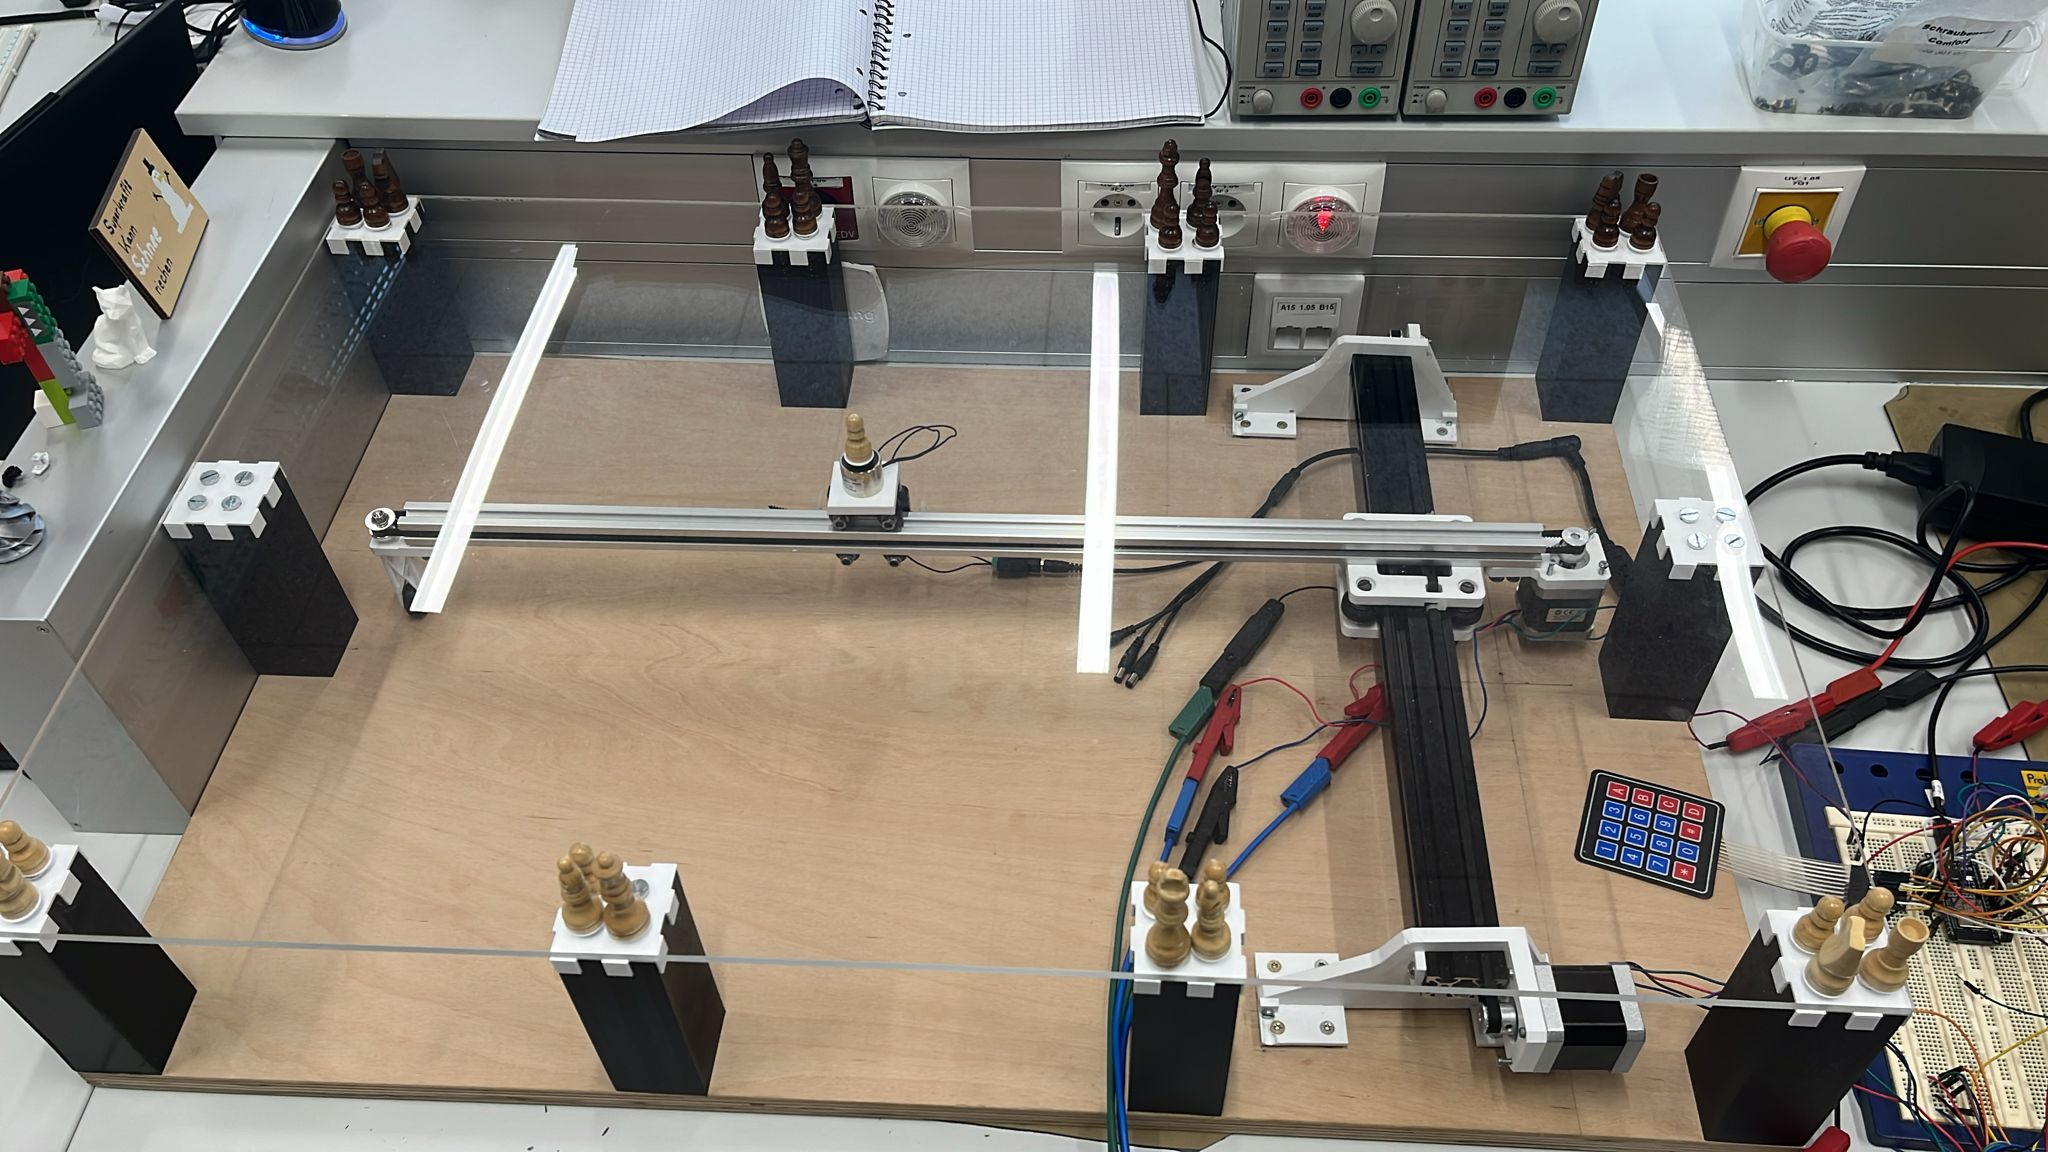
\includegraphics[width=0.95\textwidth]{images_zensiert/system_overview.jpeg}}
    \caption{Schachbot system}
    \label{fig:system}
\end{figure}

\newpage

\section*{Technical Documentation}
\section{Hardware}

\subsection{Circuit / Layout}

\subsubsection{Circuit Diagram Mainboard}
The complete schematic of the mainboard was designed in EasyEDA. It shows the ESP32
(U1) at its centre together with the two stepper-driver carriers (U4, U5), the coil
control with the MOSFET (Q1), the connectors for the two key matrices, the display and
all power rails. The detailed function of each block is explained in
Section~\ref{sec:circuit_explanation}.

\begin{figure}[H]
    \centering
    \fboxrule=1.2pt
    \fcolorbox{black}{white}{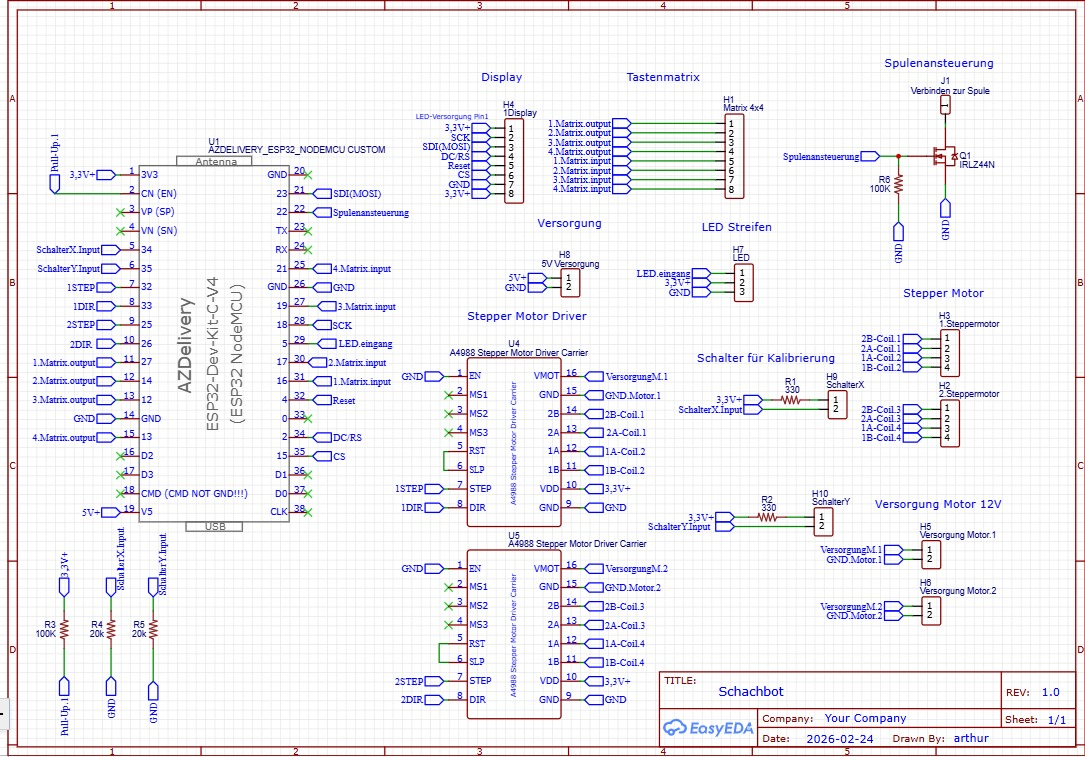
\includegraphics[width=1\textwidth]{images_zensiert/circuit_diagram_mainboard.jpeg}}
    \caption{Circuit diagram of the mainboard (EasyEDA schematic)}
    \label{fig:circuit_diagram}
\end{figure}

\newpage

\subsubsection{Assembly Plan Mainboard}
The assembly plan shows the placement of every component on the single-sided board.
It was used as a reference while soldering the parts onto the milled PCB, so that every
header, resistor and driver sits in its correct position.

\begin{figure}[H]
    \centering
    \fboxrule=1.2pt
    \fcolorbox{black}{white}{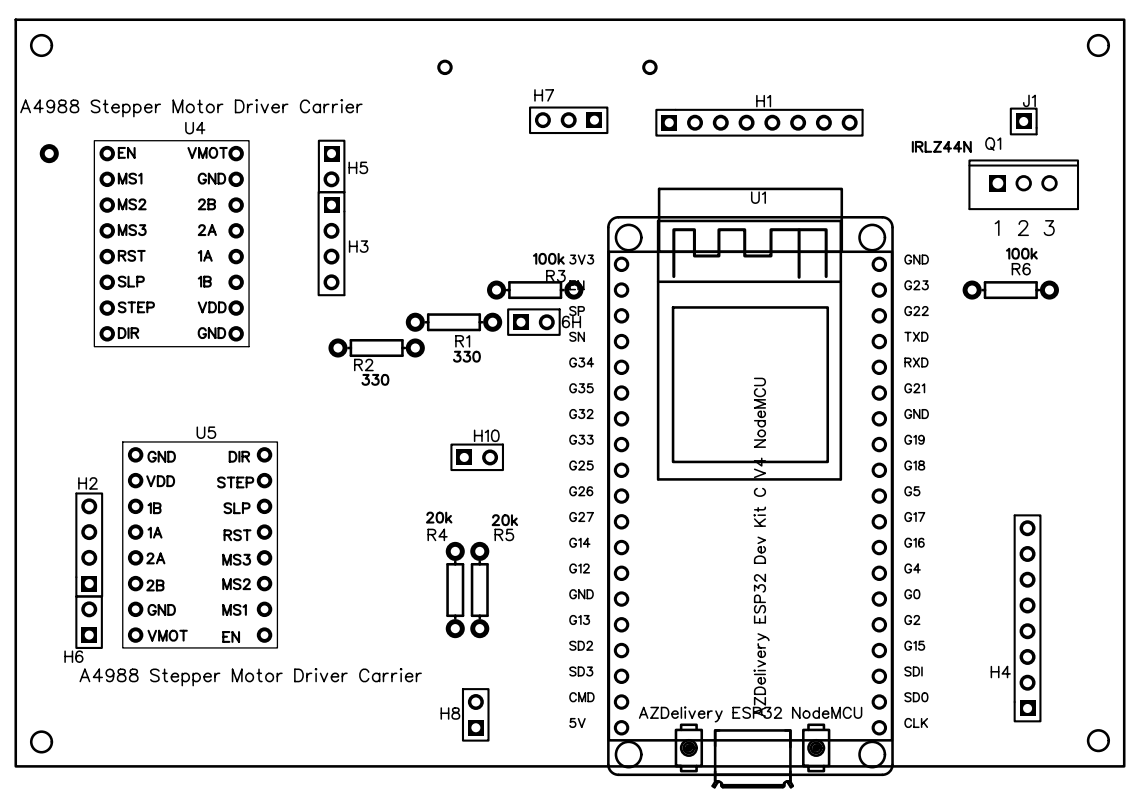
\includegraphics[width=0.85\textwidth]{images_zensiert/assembly_plan_mainboard.png}}
    \caption{Assembly / placement plan of the mainboard}
    \label{fig:assembly_plan}
\end{figure}

\subsubsection{Circuit Paths Mainboard}
This layer shows the copper traces of the single-sided, self-milled PCB. All
connections are routed on one side only, which is why the board had to be designed
carefully to avoid crossing paths. The chess-piece motif and the project label were
added to the copper layer as a small design detail.

\begin{figure}[H]
    \centering
    \fboxrule=1.2pt
    \fcolorbox{black}{white}{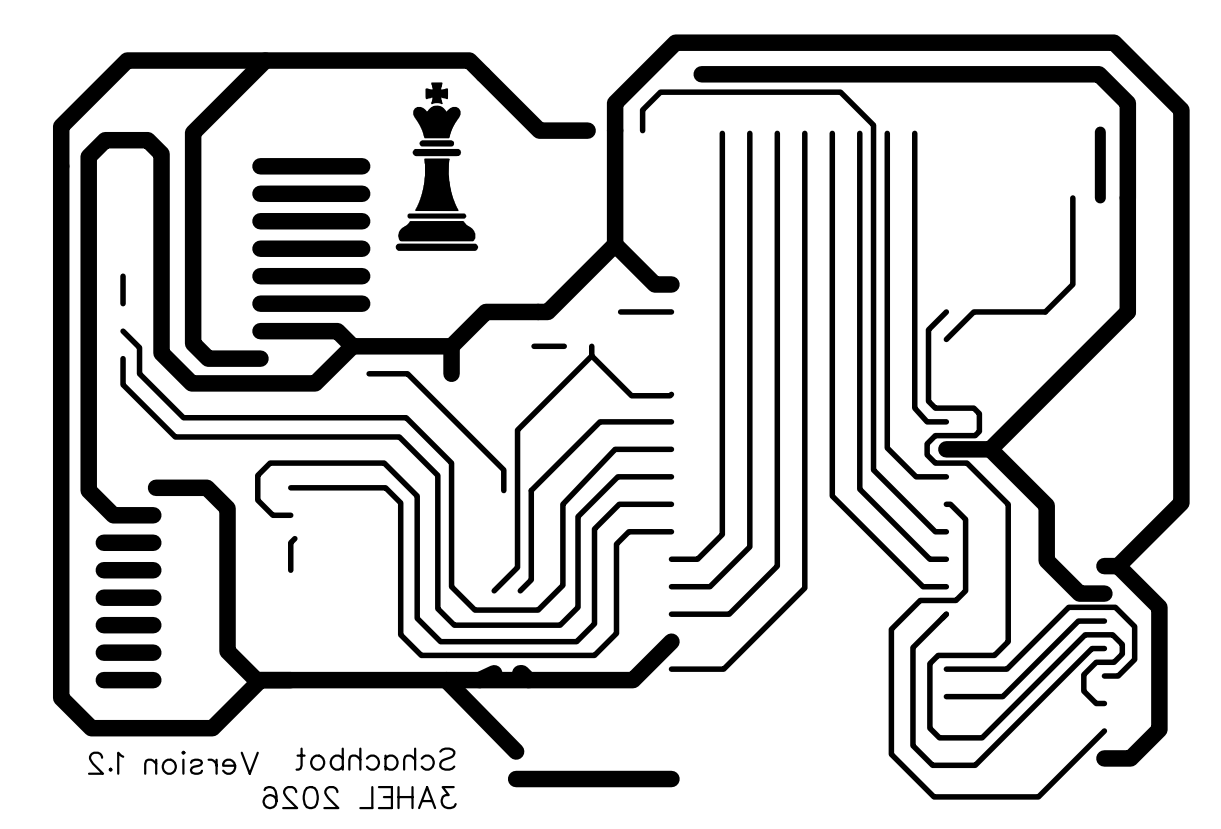
\includegraphics[width=0.8\textwidth]{images_zensiert/circuit_paths_mainboard.png}}
    \caption{Copper traces of the single-sided mainboard}
    \label{fig:circuit_paths}
\end{figure}

\newpage

\subsection{Explanation of the Circuit}
\label{sec:circuit_explanation}

\subsubsection{ESP32}
\begin{figure}[H]
    \centering
    \fboxrule=1.2pt
    \fcolorbox{black}{white}{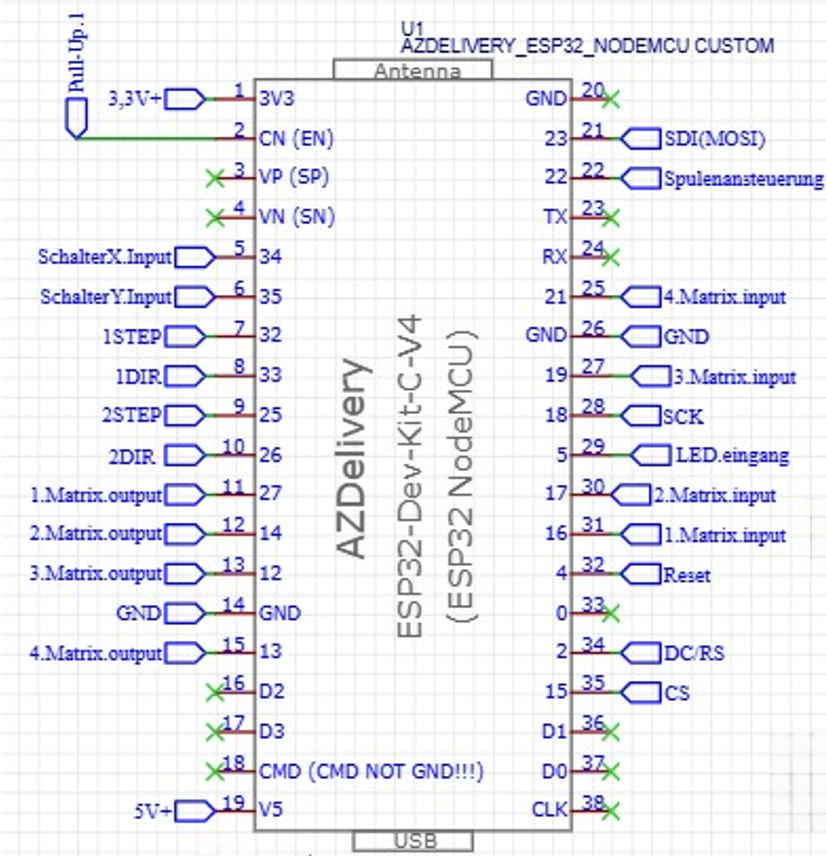
\includegraphics[width=0.55\textwidth]{images_zensiert/circuit_esp32.png}}
    \caption{ESP32 NodeMCU (U1)}
    \label{fig:circuit_esp32}
\end{figure}
The ESP32 (U1) is the central control unit of the Schachbot and coordinates all inputs
and outputs of the system. It reads the two 4×4 key matrices, runs the complete
chess-rule logic, sends the STEP and DIR signals to the two stepper drivers, switches
the electromagnet and handles the WLAN connection to the Stockfish Online API ,
Stockfish being one of the strongest chess engines in the world. We developed the
firmware in C++ using the Arduino framework.

\begin{itemize}
    \item Dual-core 240\,MHz processor with integrated Wi-Fi for the online AI mode
    \item Enough GPIOs for both stepper drivers, the display, the coil and the homing
          switches
    \item 5\,V logic level, supplied from the 5\,V rail through the on-board regulator
\end{itemize}

\subsubsection{Motor Drivers Output}
\begin{figure}[H]
    \centering
    \fboxrule=1.2pt
    \fcolorbox{black}{white}{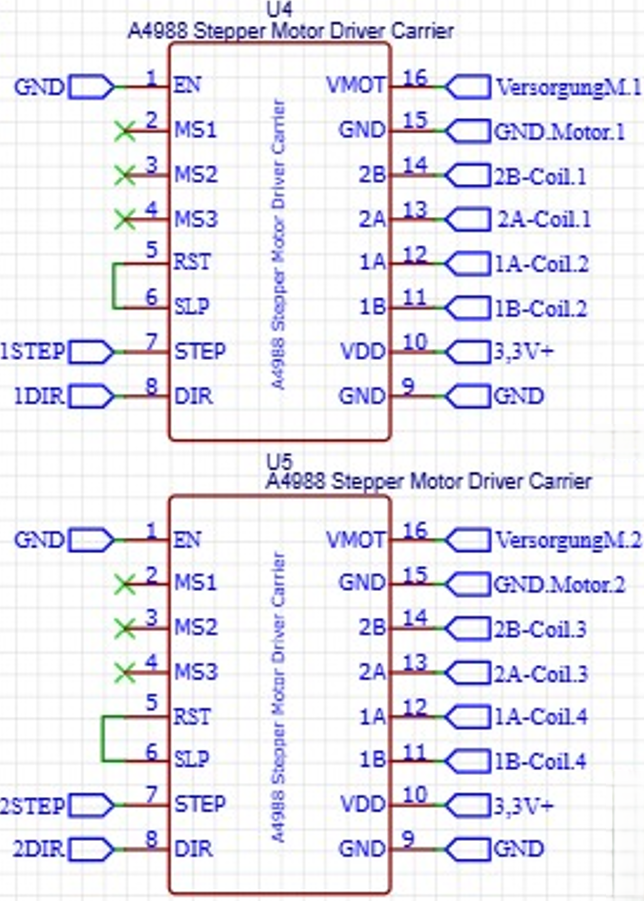
\includegraphics[width=0.5\textwidth]{images_zensiert/circuit_motor_drivers.png}}
    \caption{A4988 stepper motor drivers (U4, U5)}
    \label{fig:circuit_motor_drivers}
\end{figure}
The two stepper motors of the X- and Y-axis are driven by two A4988 stepper-driver
carriers (U4, U5). The ESP32 only outputs the low-power STEP and DIR signals , the
driver itself generates the high coil currents for the motor.

\begin{itemize}
    \item One driver per axis: U4 is controlled by 1STEP/1DIR, U5 by 2STEP/2DIR from
          the ESP32
    \item Coil outputs 1A/1B and 2A/2B drive the two motor windings of each stepper
    \item VMOT = 12\,V motor supply, VDD = 5\,V logic supply
\end{itemize}

\subsubsection{Display Input}
\begin{figure}[H]
    \centering
    \fboxrule=1.2pt
    \fcolorbox{black}{white}{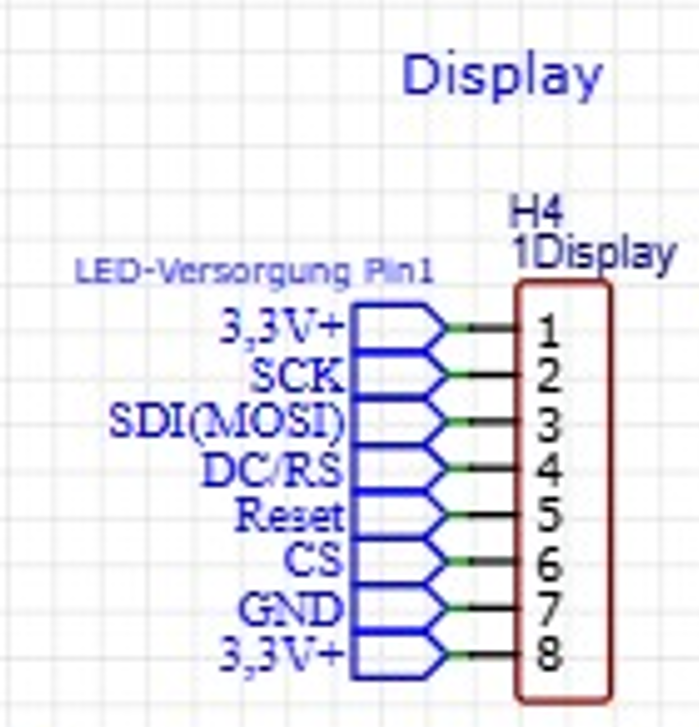
\includegraphics[width=0.4\textwidth]{images_zensiert/circuit_display.png}}
    \caption{Display connection (H4)}
    \label{fig:circuit_display}
\end{figure}
The LC-display shows whose turn it is, the current board state as the controller
``sees'' it, and status messages such as ``Start Programm'' or error outputs. It is
connected to the ESP32 over header H4 via its control lines (SCK, SDI(MOSI), DC/RS, CS,
Reset) and powered from the 5\,V rail.

\begin{itemize}
    \item Serial connection to the ESP32 (SCK, MOSI, DC/RS, CS, Reset)
    \item Powered from 5\,V with a common ground
    \item Output only , used purely to give the players visual feedback
\end{itemize}

\newpage

\subsubsection{Limit / Homing Switches Input}
\begin{figure}[H]
    \centering
    \fboxrule=1.2pt
    \fcolorbox{black}{white}{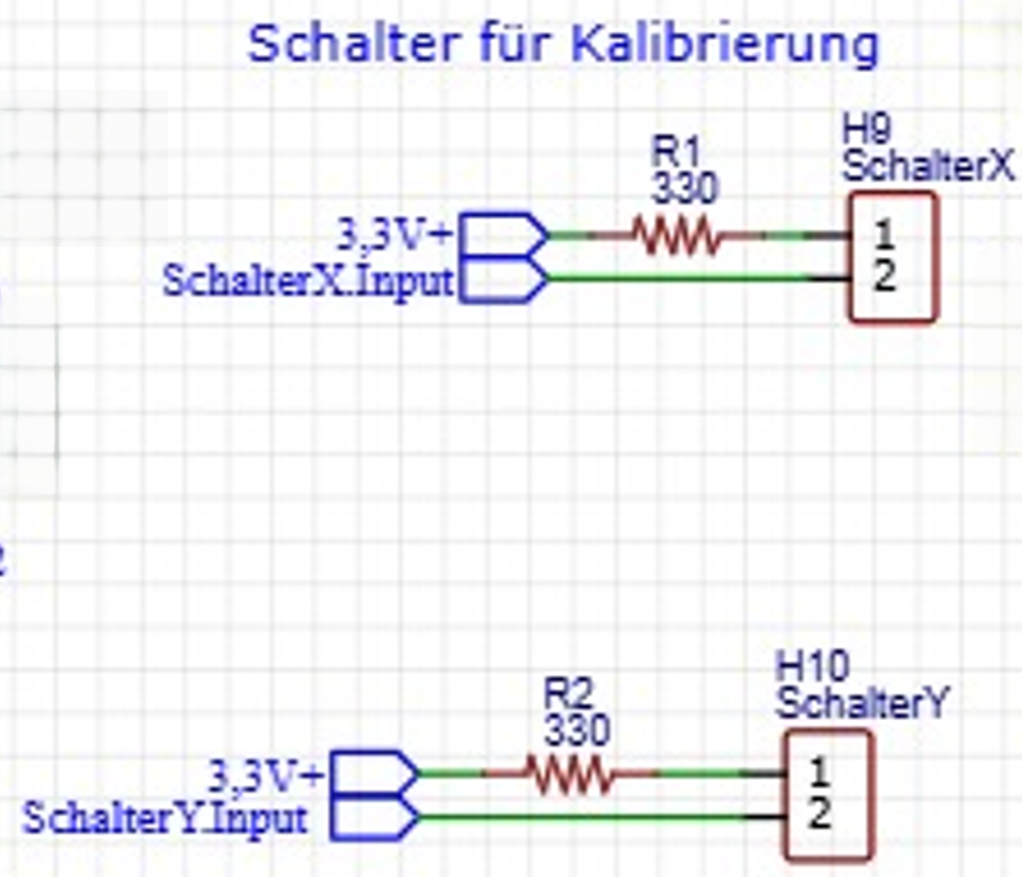
\includegraphics[width=0.5\textwidth]{images_zensiert/circuit_limit_switches.png}}
    \caption{Homing / limit switches (H9, H10)}
    \label{fig:circuit_limit_switches}
\end{figure}
The two switches (SchalterX on H9 and SchalterY on H10) are used to home the gantry at
start-up and act as limit inputs for the X- and Y-axis. On power-up the controller does
not know where the magnet currently sits, so it drives each axis until its switch is
triggered. That point is defined as the zero position (X=0, Y=0), and from there the
ESP32 can reach every square by counting steps. Without this homing run every movement
would be inaccurate, because the starting point would be unknown.

\begin{itemize}
    \item Series resistors R1/R2 (330\,$\Omega$) protect the GPIO inputs
    \item Pull-down resistors R3 (100\,k), R4/R5 (20\,k) keep the inputs at a stable,
          defined logic level
    \item Zero position of the gantry is set from these switches on every power-up
          (homing)
\end{itemize}

\newpage

\subsubsection{Coil Control}
\begin{figure}[H]
    \centering
    \fboxrule=1.2pt
    \fcolorbox{black}{white}{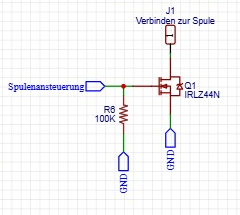
\includegraphics[width=0.45\textwidth]{images_zensiert/circuit_coil.png}}
    \caption{Coil control with MOSFET Q1}
    \label{fig:circuit_coil}
\end{figure}
The electromagnet (Spule) drags the chess pieces across the board. It is switched by an
N-channel MOSFET (Q1, IRLZ44N), which only turns the coil on and off. The positive
terminal of the coil is permanently connected to the supply via J1, while the MOSFET
switches the ground side. To do this, the ESP32 only drives the gate of the MOSFET.

\begin{itemize}
    \item N-channel MOSFET Q1 (IRLZ44N) switches the ground connection of the coil
    \item J1 is the positive terminal of the coil (permanently tied to the supply)
    \item Pull-down resistor R6 (100\,k) pulls the gate to GND while the ESP32 drives
          nothing, so the coil stays safely off at power-up
\end{itemize}

\subsubsection{Power Supply}
\begin{figure}[H]
    \centering
    \fboxrule=1.2pt
    \fcolorbox{black}{white}{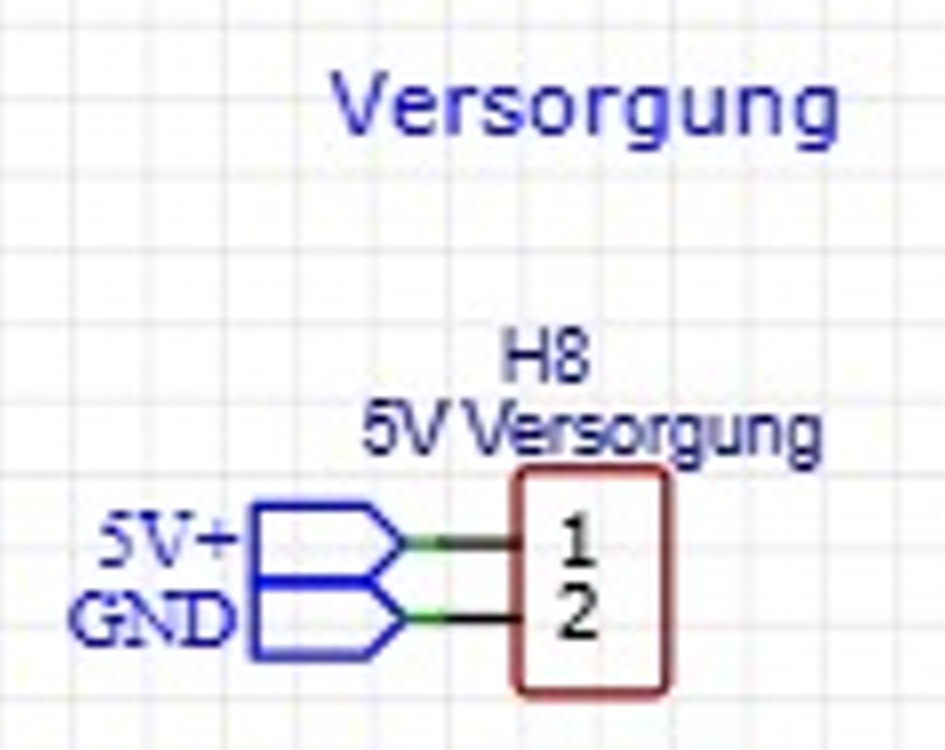
\includegraphics[width=0.4\textwidth]{images_zensiert/circuit_power.png}}
    \caption{5\,V supply connection (H8)}
    \label{fig:circuit_power}
\end{figure}
The whole system is supplied from a 24\,V power supply connected to the 230\,V wall
socket. From there the voltage is distributed and stepped down to the levels the
individual subsystems need. The high-current rail feeds the stepper motors and the
electromagnet, while a separate logic rail supplies the ESP32, the display and the key
matrices.

\begin{itemize}
    \item 12\,V motor rail (H5/H6) supplies VMOT of the stepper drivers and the
          electromagnet
    \item 5\,V rail (H8) feeds the ESP32, the display and the LED strip (H7)
    \item Separated supplies: keeping the motor/coil currents away from the logic lines
          keeps the signals clean
\end{itemize}

\newpage

\section{3D-Design}

\subsection{Gantry 3D-Designs}

\subsubsection{Complete 2D-Gantry}

\begin{figure}[H]
    \centering
    \fboxrule=1.2pt
    \fcolorbox{black}{white}{\includegraphics[width=0.85\textwidth]{images_zensiert/2D_Gantry.png}}
    \caption{Complete 2D-Gantry}
    \vspace{5pt}
    \begin{minipage}{0.9\textwidth}
        \textbf{2D-Gantry Overview:} \\
        The 2D gantry is the mechanical heart of the Schachbot. It moves the electromagnet
        in the X- and Y-direction underneath the board so that any piece can be dragged to
        any square. Two stepper motors drive the axes via toothed pulleys and timing belts:
        one motor moves the long cross-beam (X-axis), the second is carried along on the
        beam and moves the carriage with the magnet (Y-axis). The axes are built from
        aluminium profiles, and every motor, pulley and carriage is held by a custom
        3D-printed bracket. All printed parts are shown in detail in the following sections.
    \end{minipage}
\end{figure}
\newpage

\subsubsection{Gantry X-Axis Mounts}

\begin{figure}[H]
    \centering
    \fboxrule=1.2pt
    \fcolorbox{black}{white}{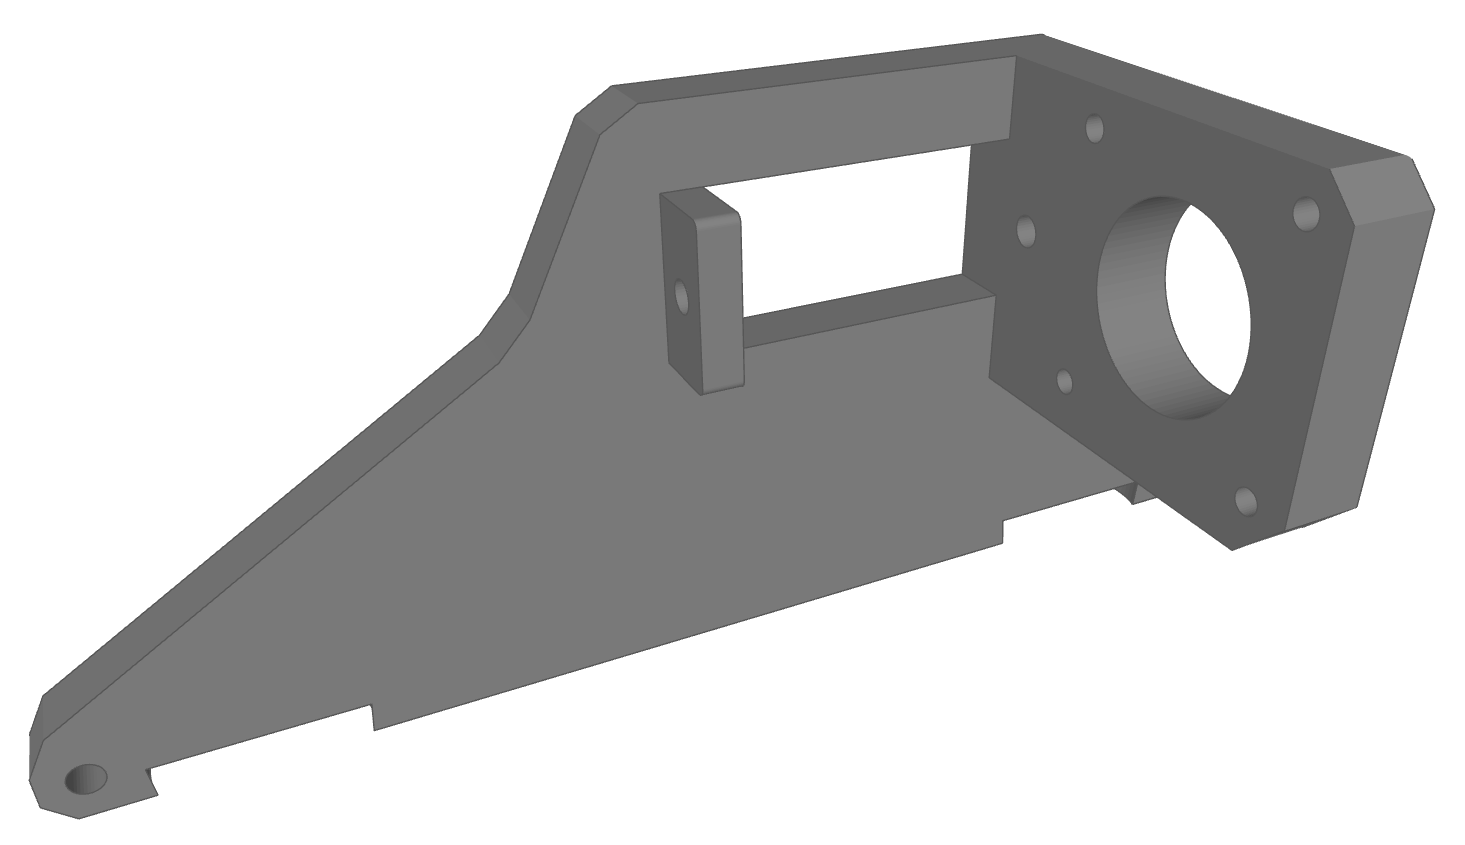
\includegraphics[width=0.45\textwidth]{images_zensiert/X_achse_motorhalterung.png}}
    \hfill
    \fcolorbox{black}{white}{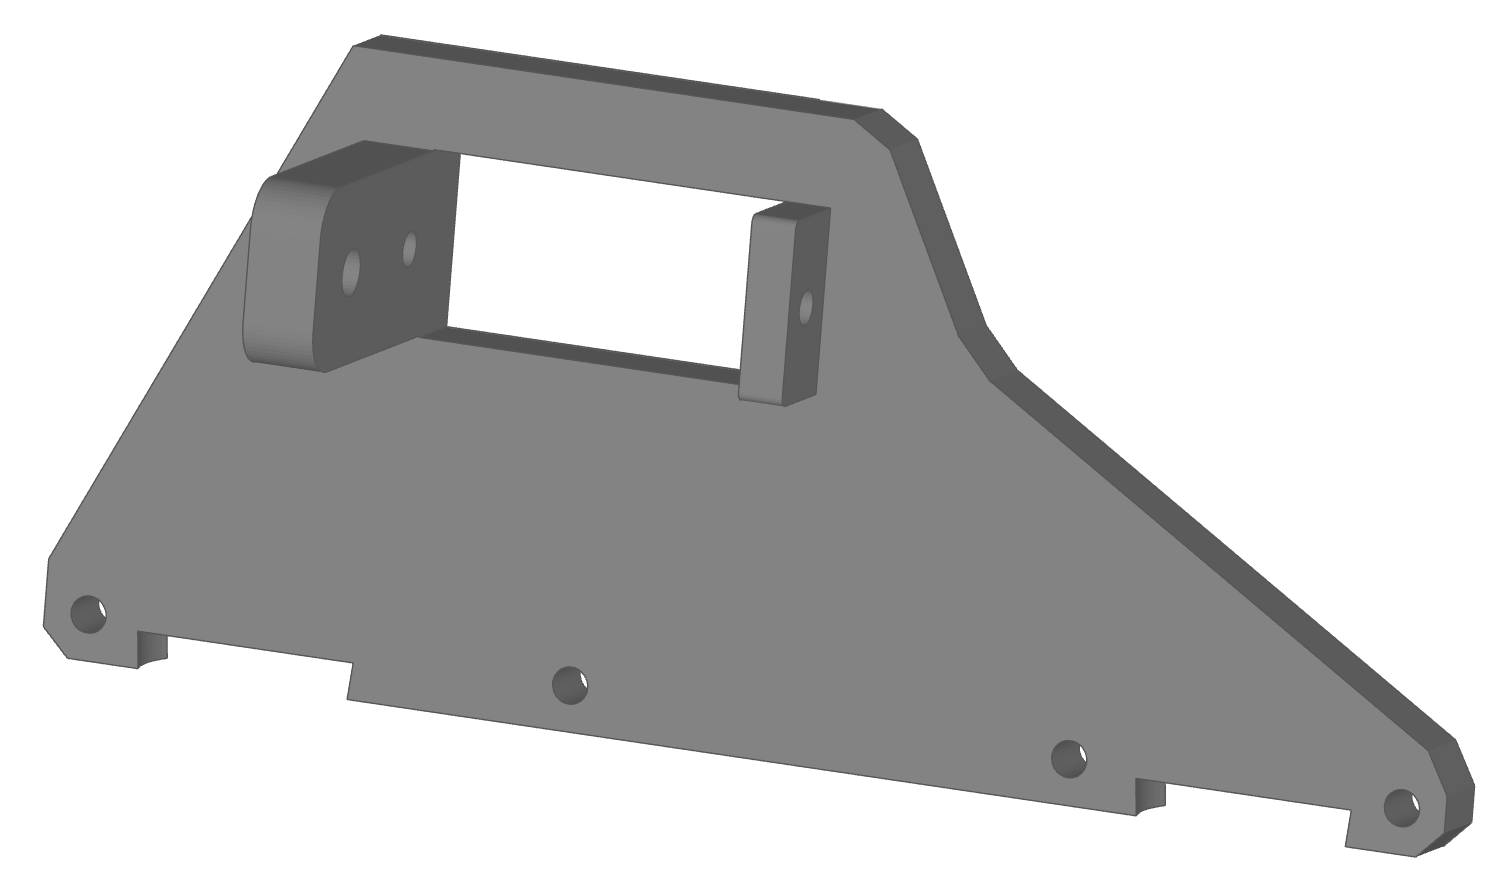
\includegraphics[width=0.45\textwidth]{images_zensiert/X_achse_zahnradhalterung.png}}
    \caption{X-axis: motor mount (left) and pulley/idler mount (right)}
    \vspace{5pt}
    \begin{minipage}{0.9\textwidth}
        \textbf{X-Axis Mounts:} \\
        The X-axis is driven from one side and runs over an idler on the other side.
        \begin{itemize}
            \item \textbf{Motor mount (left):} holds the stepper motor of the X-axis. The
                  large circular cut-out fits the motor body, the four holes around it take
                  are for the mounting screws, and the two extra holes fix the bracket to the
                  aluminium profile.
            \item \textbf{Pulley / idler mount (right):} carries the idler bearing on the
                  opposite end of the X-axis. The belt runs around this idler, and the two
                  through-holes screw the bracket onto the profile.
        \end{itemize}
        Together they tension the belt and convert the motor rotation into a clean linear
        movement of the cross-beam.
    \end{minipage}
\end{figure}

\vspace{20pt}

\subsubsection{Axis Transition}
% 1 image: nächste_achse_halterung.png
\begin{figure}[H]
    \centering
    \fboxrule=1.2pt
    \fcolorbox{black}{white}{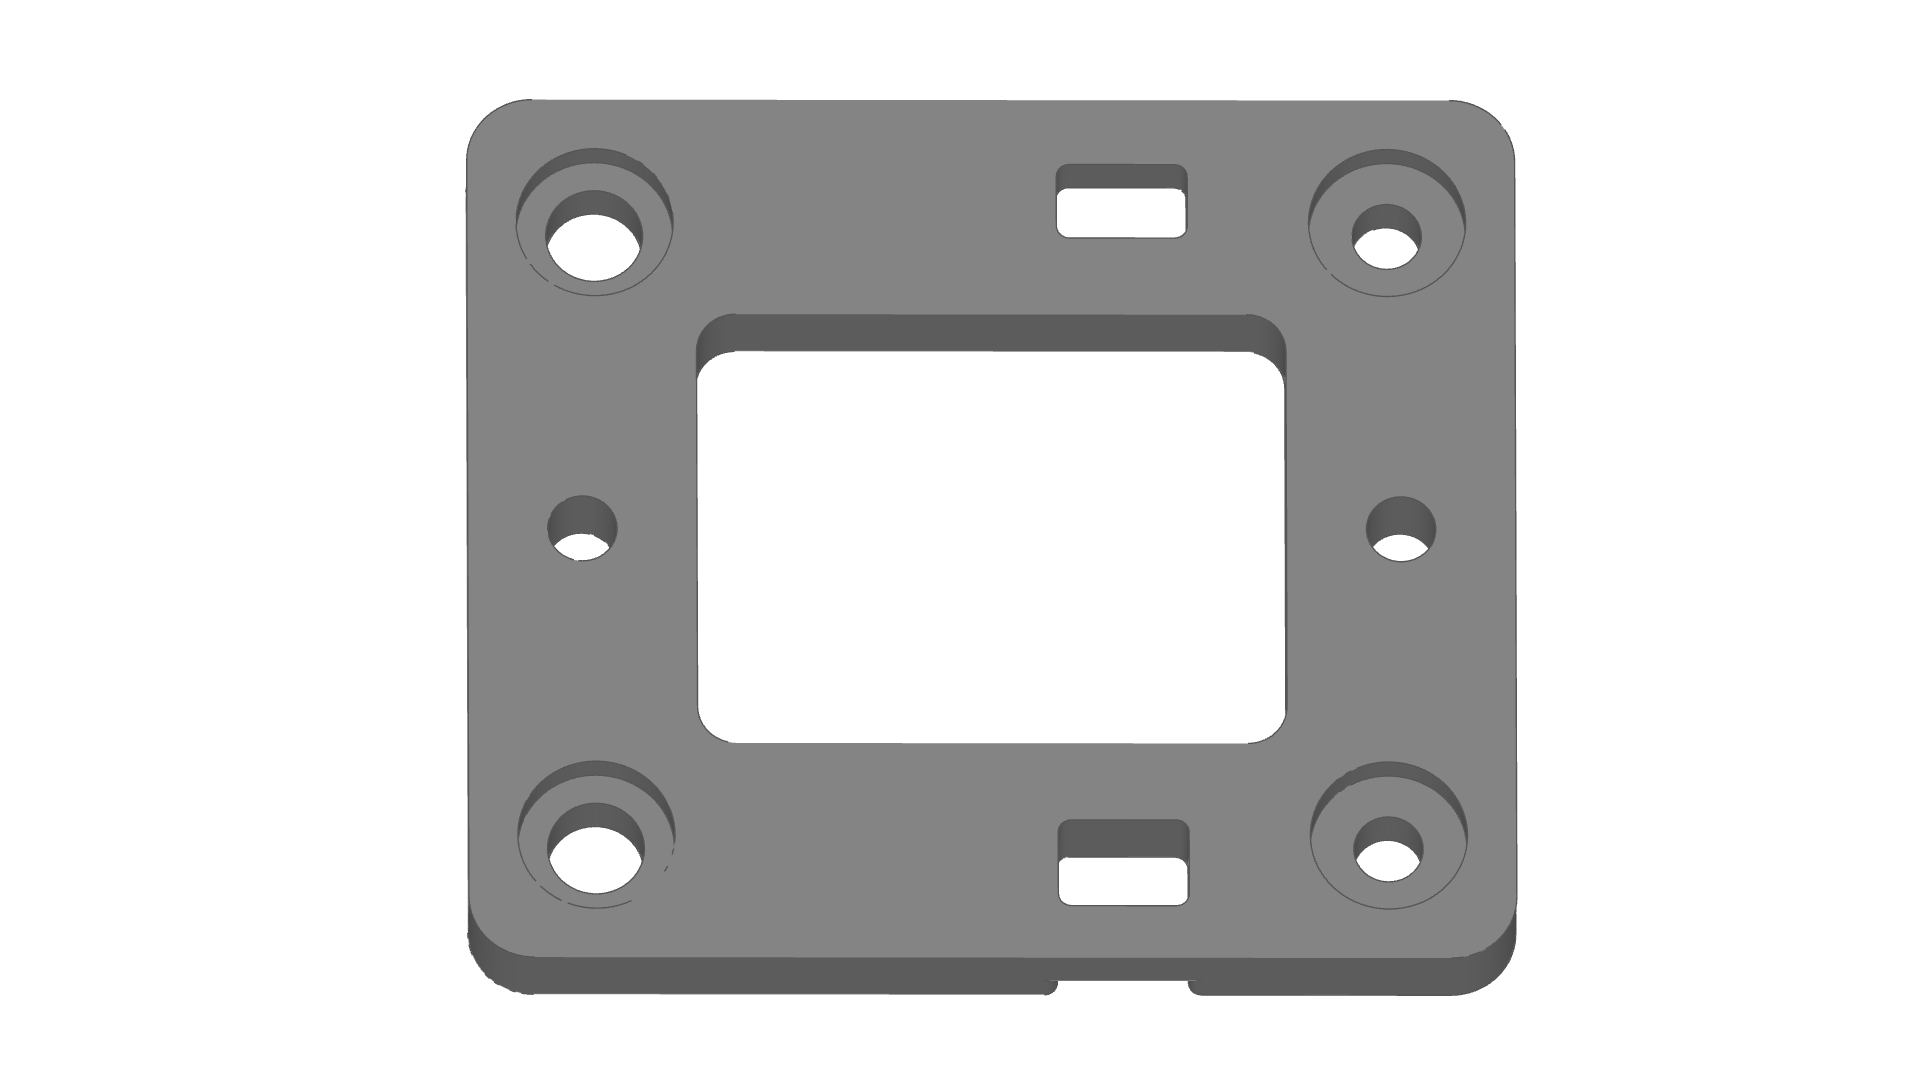
\includegraphics[width=0.55\textwidth]{images_zensiert/nächste_achse_halterung.png}}
    \caption{Transition plate between the X- and Y-axis}
    \vspace{5pt}
    \begin{minipage}{0.9\textwidth}
        \textbf{Axis Transition:} \\
        This carriage plate is the link between the two axes: it rides on the X-axis and at
        the same time carries the complete Y-axis on top. The four countersunk holes mount
        the rollers/bearings that run on the profile, the two centre holes connect to the
        Y-axis structure, and the small slots are used to route and fix the timing belt.
        Because it carries the whole second axis, this part has to be stiff and precisely
        printed so the movement stays free of play.
    \end{minipage}
\end{figure}
\newpage

\subsubsection{Gantry Y-Axis Mounts}

    \begin{figure}[H]
        \centering
        \fboxrule=1.2pt
        \fcolorbox{black}{white}{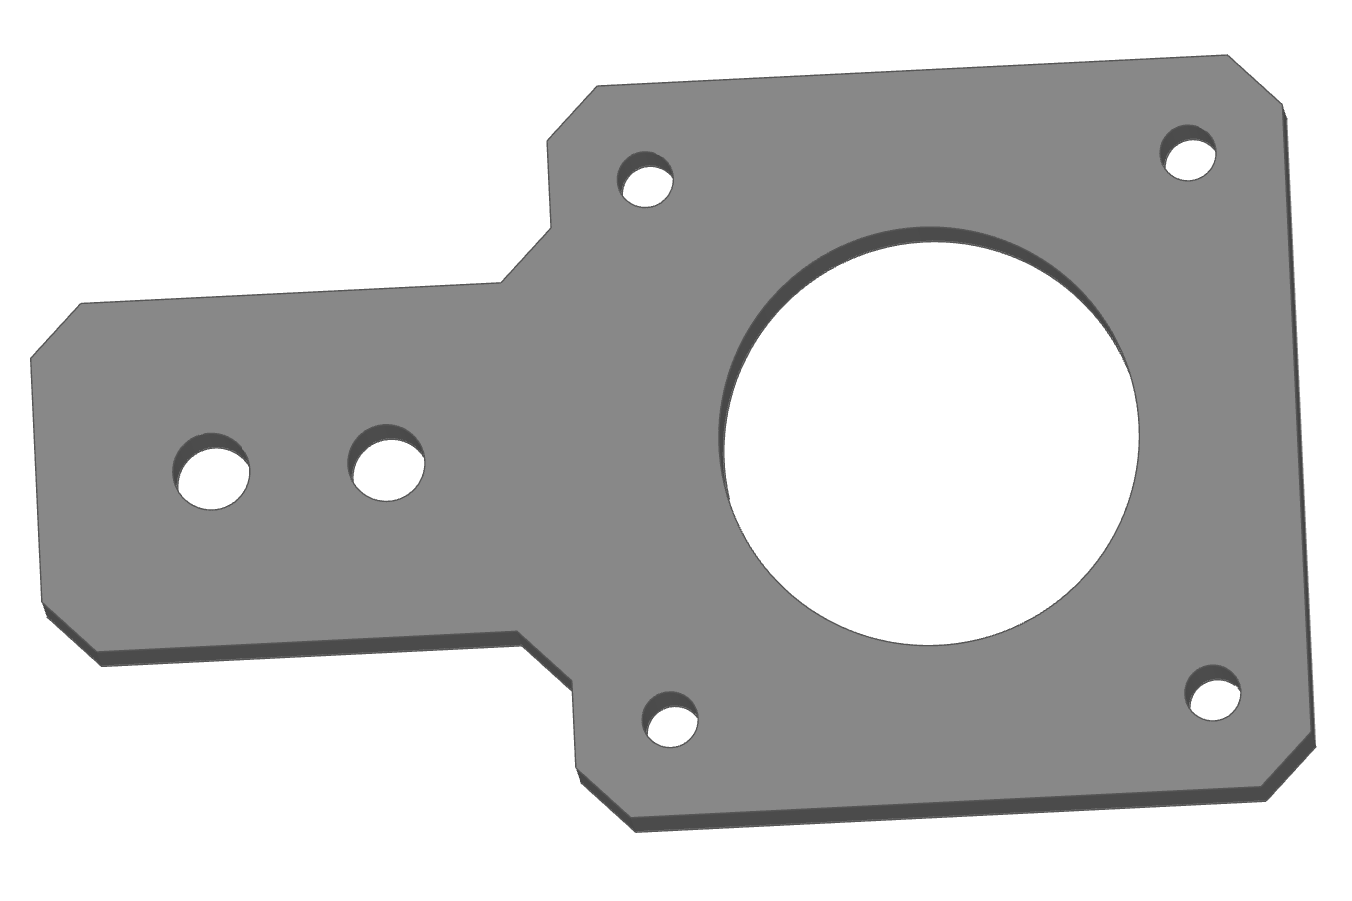
\includegraphics[width=0.45\textwidth]{images_zensiert/Y_achse_moterhalterung.png}}
        \hfill
        \fcolorbox{black}{white}{
\includegraphics[width=0.45\textwidth]{images_zensiert/Y_achse_zahnradhalterung.png}}
        \caption{Y-axis: motor mount (left) and pulley/idler mount (right)}
        \vspace{5pt}
        \begin{minipage}{0.9\textwidth}
            \textbf{Y-Axis Mounts:} \\
            The Y-axis sits on top of the transition plate and works the same way as the X-axis,
            but with wedge-shaped brackets that give the tall structure extra stability.
            \begin{itemize}
                \item \textbf{Motor mount (left):} the wedge bracket holds the Y-axis stepper
                      motor; the round cut-out and the surrounding holes take the motor and its
                      screws, while the long flat base bolts onto the profile.
                \item \textbf{Pulley / idler mount (right):} mirrors the motor mount on the
                      opposite end and holds the idler for the Y-belt, keeping the belt tensioned
                      across the axis.
            \end{itemize}
        \end{minipage}
    \end{figure}

    \vspace{20pt}

\subsubsection{Custom Carriage}
\begin{figure}[H]
    \centering
    \fboxrule=1.2pt
    \fcolorbox{black}{white}{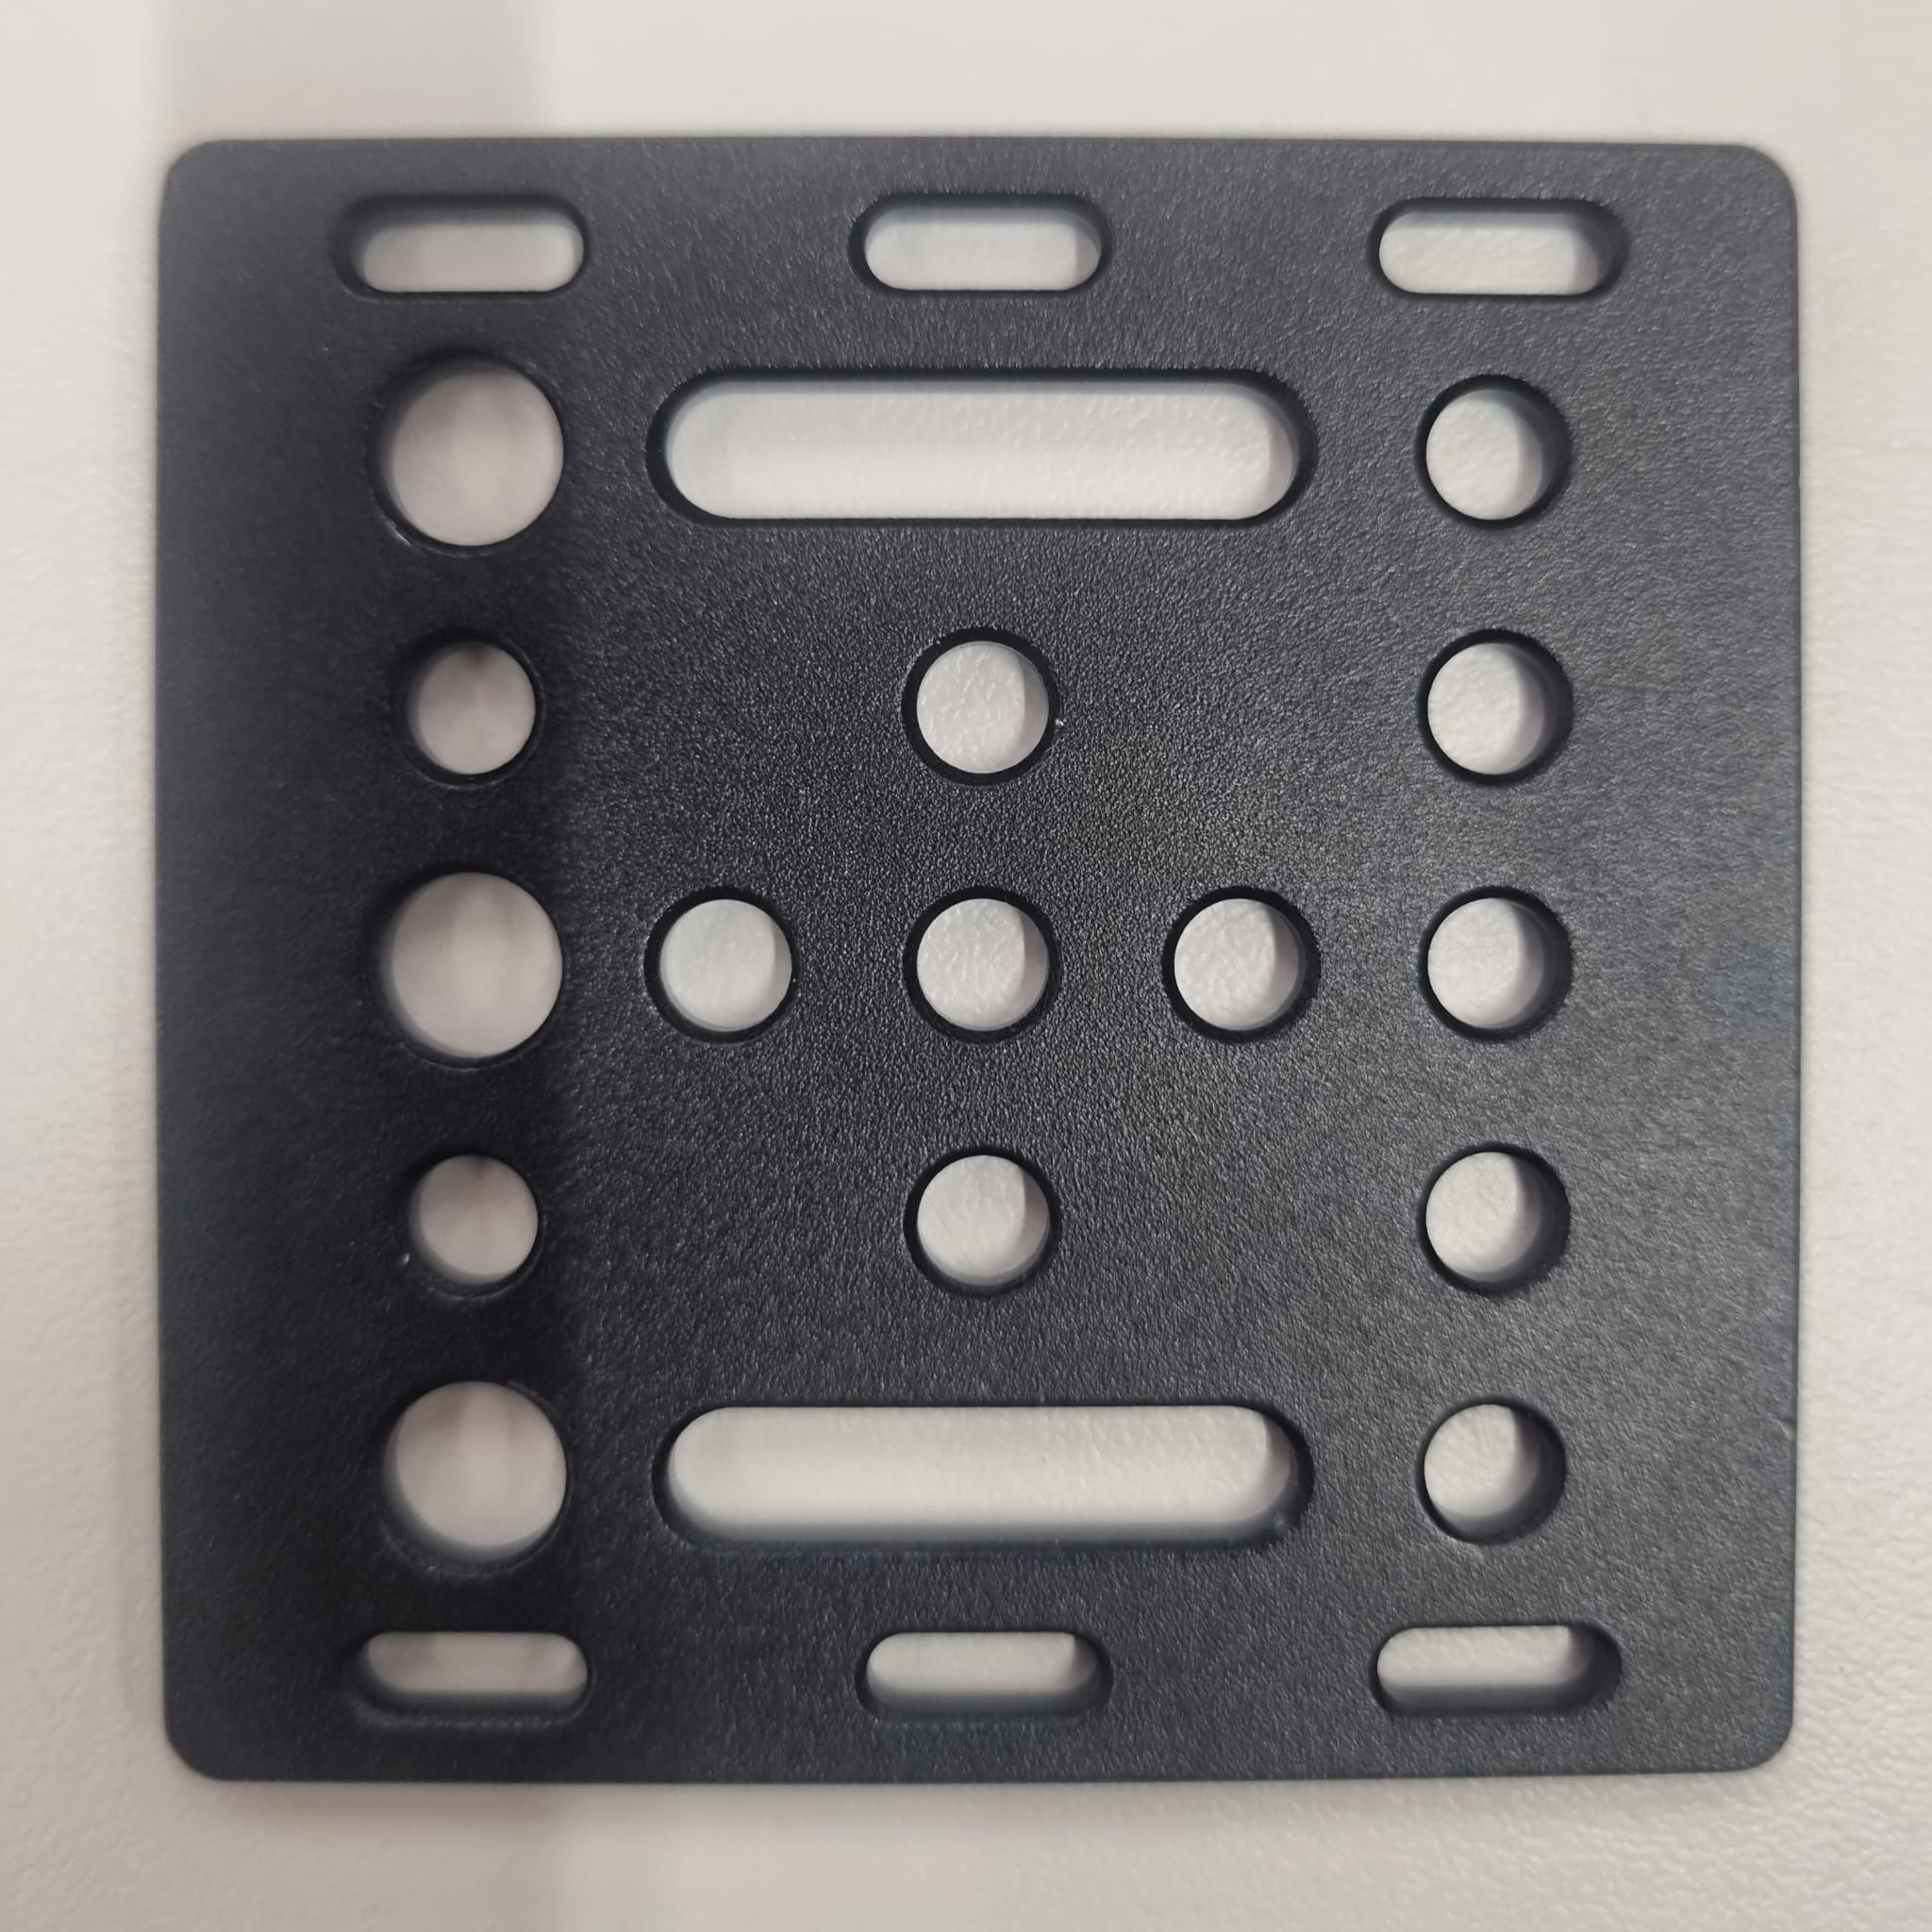
\includegraphics[width=0.35\textwidth]{images_zensiert/custom_carriage.jpeg}}
    \caption{Custom carriage plate of the Y-axis}
    \vspace{5pt}
    \begin{minipage}{0.9\textwidth}
        \textbf{Custom Carriage:} \\
        The carriage is the moving part of the Y-axis. Like the X-to-Y transition plate it
        is mounted on the smaller aluminium profile and rolls along it on its bearings. The
        many holes and slots let us bolt on the rollers, the belt clamp and the
        electromagnet bracket in different positions, which made it easy to align everything
        during assembly. This carriage carries the electromagnet that actually drags the
        chess pieces across the board.
    \end{minipage}
\end{figure}

\newpage


\subsection{Casing 3D-Designs}

\subsubsection{Custom Display Case}
% 2 images_zensiert: display_casing.png + display_deckel.png
\begin{figure}[H]
    \centering
    \fboxrule=1.2pt
    \fcolorbox{black}{white}{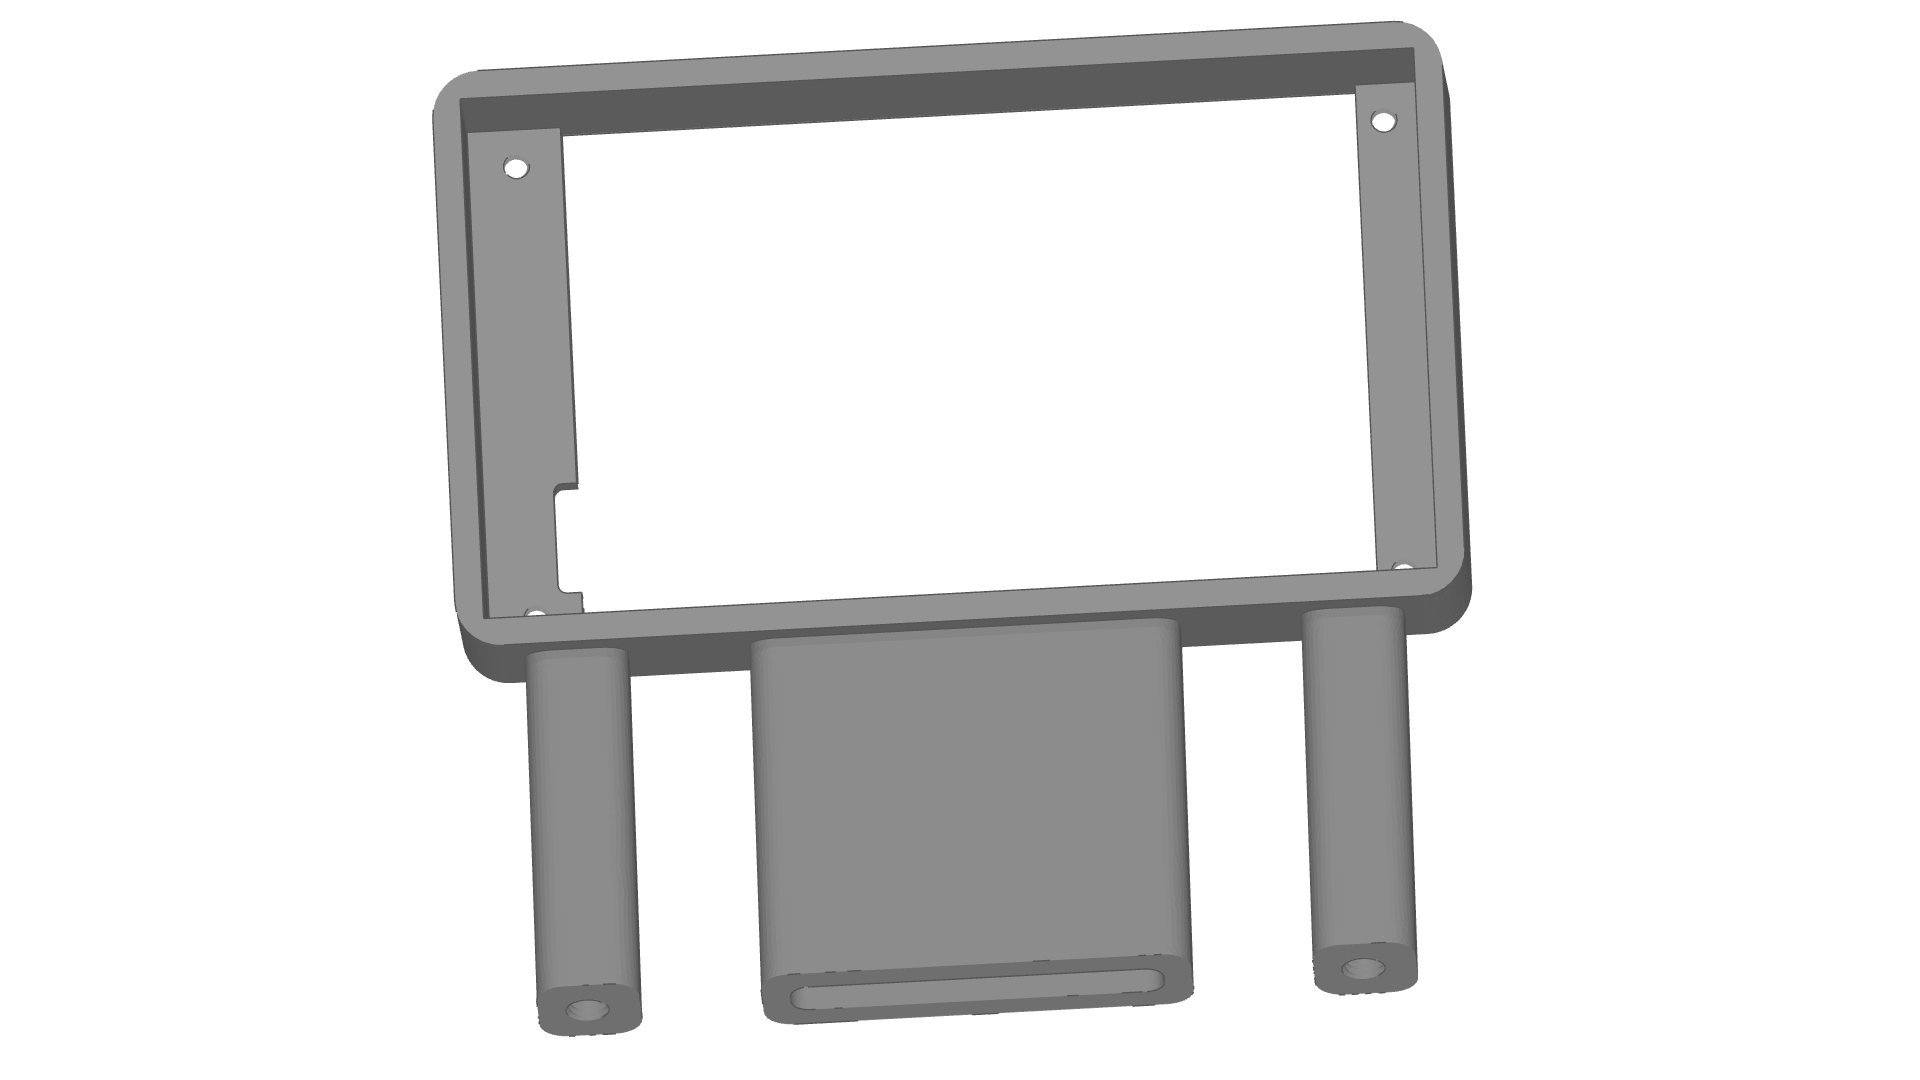
\includegraphics[width=0.45\textwidth]{images_zensiert/display_casing.png}}
    \hfill
    \fcolorbox{black}{white}{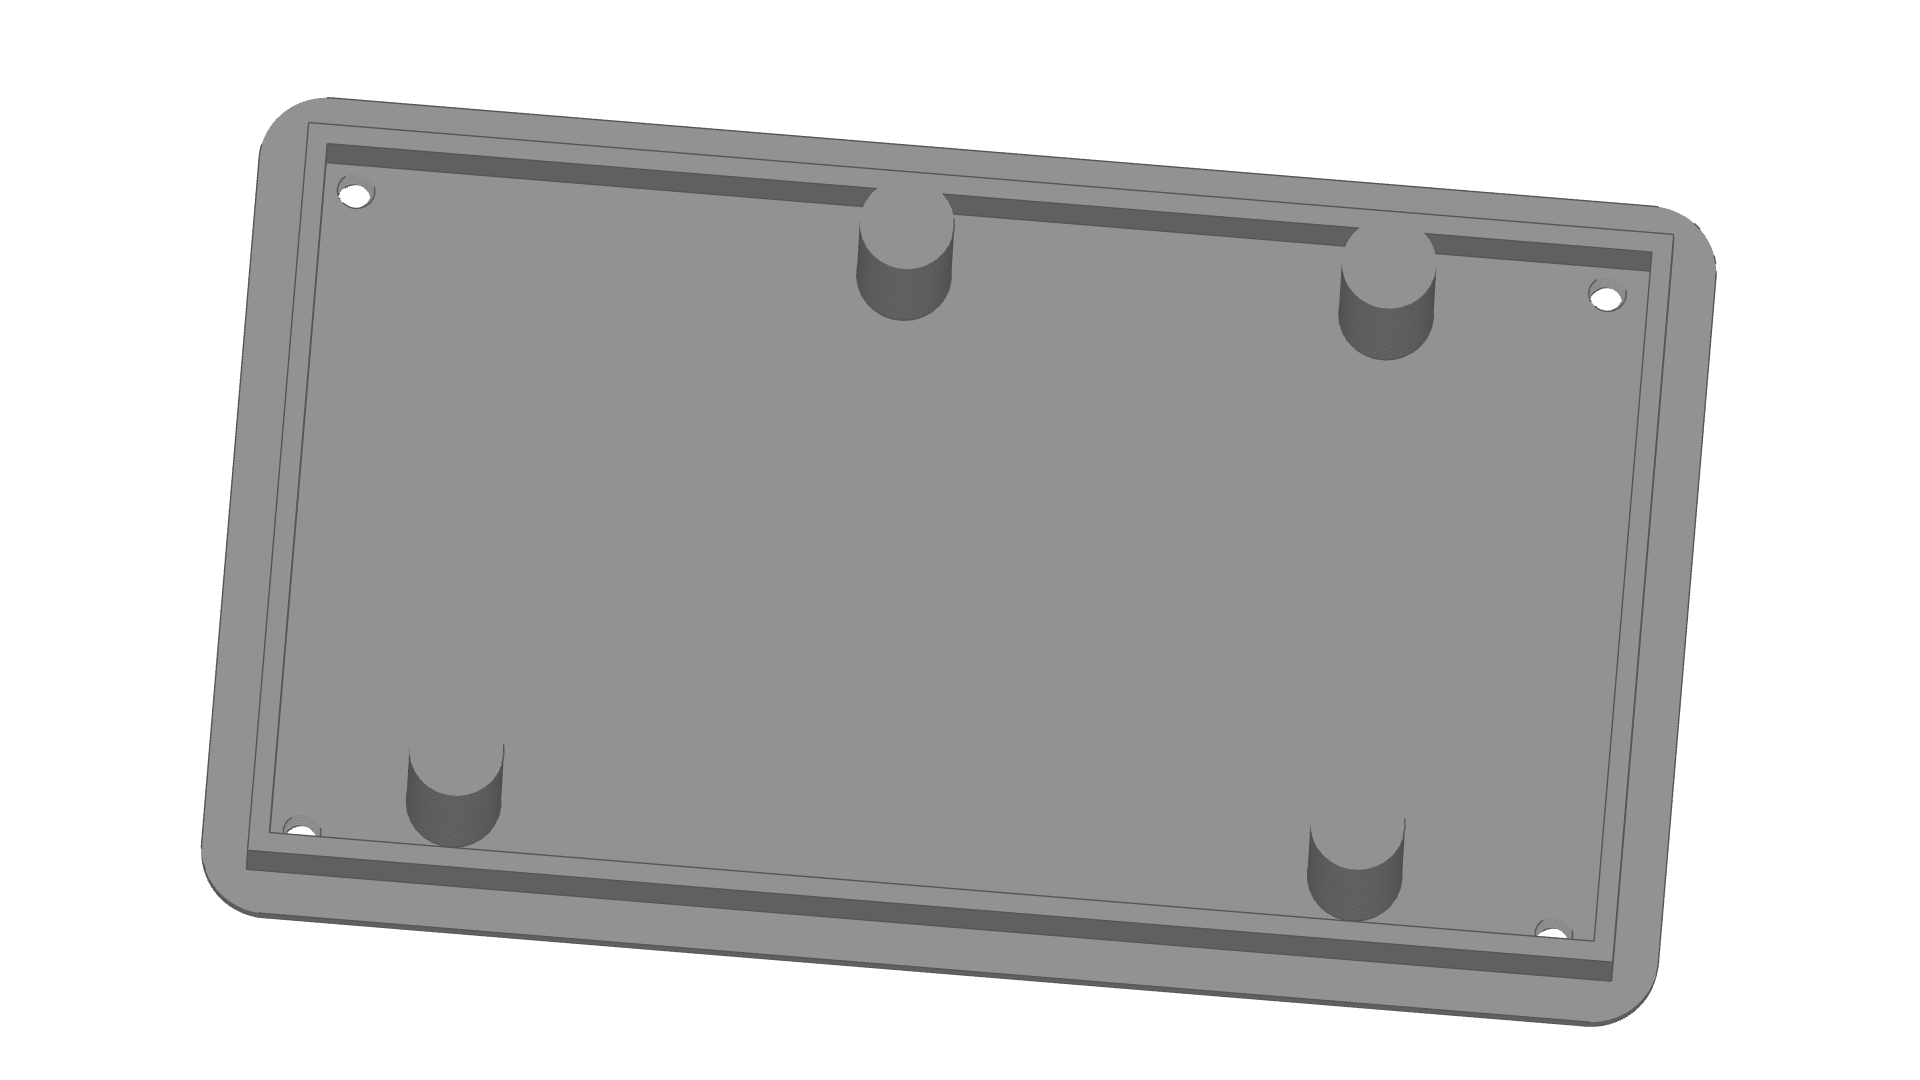
\includegraphics[width=0.45\textwidth]{images_zensiert/display_deckel.png}}
    \caption{Display case: front stand (left) and back cover (right)}
    \vspace{5pt}
    \begin{minipage}{0.9\textwidth}
        \textbf{Display Case:} \\
        The display is housed in a custom two-part case that stands on the table at a
        viewing angle thats normal to both players.
        \begin{itemize}
            \item \textbf{Stand (left):} the angled base holds the display upright and
                  tilted towards the player, with a cut-out at the bottom for the cable.
            \item \textbf{Back cover (right):} closes the case from behind. The corner holes
                  screw the two halves together, and the small pins inside fix the display
                  board in place so it cannot shift.
        \end{itemize}
    \end{minipage}
\end{figure}

\vspace{20pt}

\subsubsection{Custom Tastenmatrix Case}
% 1 image: tastenmatrix_halterung.png
\begin{figure}[H]
    \centering
    \fboxrule=1.2pt
    \fcolorbox{black}{white}{
\includegraphics[width=0.55\textwidth]{images_zensiert/tastenmatrix_halterung.png}}
    \caption{Holder for the key matrix}
    \vspace{5pt}
    \begin{minipage}{0.9\textwidth}
        \textbf{Tastenmatrix Holder:} \\
        This frame holds one of the 4×4 key matrices. The rectangular opening fits the
        keypads wires perfectly so the wires can get to the circut via the hole behin the 4x4 key matrices, the corner holes fix the matrix to the frame, and
        the two legs underneath raise it to the right height and keep it stable while
        a player enters a move.
    \end{minipage}
\end{figure}
\newpage

\subsubsection{Custom Support Pillar}
% 1 image: stüze.png
\begin{figure}[H]
    \centering
    \fboxrule=1.2pt
    \fcolorbox{black}{white}{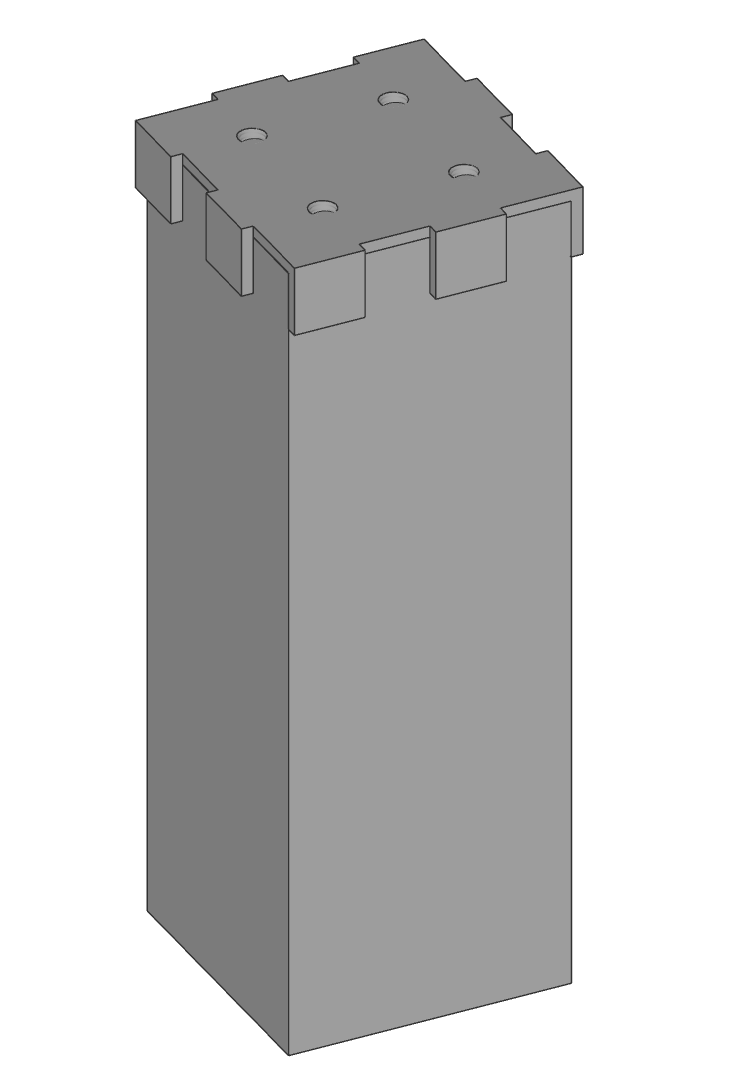
\includegraphics[width=0.4\textwidth]{images_zensiert/stüze.png}}
    \caption{Support pillar for the playing field}
    \vspace{5pt}
    \begin{minipage}{0.9\textwidth}
        \textbf{Support Pillar:} \\
        Ten of these hollow pillars carry the plexiglass playing field above the gantry and are fixed in place with screws through the holes. The screw holes on the bottom bolt everything onto the strong wooden base plate, and the pillars' height defines the gap in which the gantry and the electromagnet move underneath the board.
    \end{minipage}
\end{figure}

\vspace{30pt}

\subsection{More Information on the 3D Design}

Of course there were many more small 3D-printed parts in the project, for example little
holders for the wiring, mounts for the DC-DC converters and supports for the circuit board / Gantry Y-axis.
The parts shown above are the most important and most complex ones and best represent the
mechanical design work behind the Schachbot.



\newpage
 
\section{Program}

The program is split into several independent sections, each implemented as its own
class:

\begin{itemize}
    \item Gantry control (including the coil activation)
    \item Display control
    \item Key matrix I/O
    \item Chess rules (including the offline bot)
    \item Chess API (online moves)
    \item Setting the WLAN password (website)
\end{itemize}

A central ``Main File'' coordinates the different sections and ensures a clean program
flow.

\begin{figure}[H]
    \centering
    \fboxrule=1.2pt
    \fcolorbox{black}{white}{\includegraphics[width=0.95\textwidth]{images_zensiert/programm_structure.png}}
    \caption{Program structure: each subsystem is implemented as its own class
        (\texttt{.cpp}/\texttt{.h} pair), tied together by \texttt{main.cpp}}
    \label{fig:program_structure}
\end{figure}

\newpage

\subsection{Gantry Movement / Coil Activation}

The class \texttt{Gantry} is a wrapper around the imported \texttt{AccelStepper} class.

\subsubsection*{Homing (Zeroing)}
On the axes of the gantry there are switches that check whether the X- or Y-position of
the gantry is equal to zero. When the function \texttt{MoveToZero()} is called, the
program switches into the \emph{MoveToZero} mode and all other tasks are interrupted
until the zero position is reached.

\subsubsection*{Move from one field to another}
The function \texttt{goTo(Koordinate start, Koordinate ende)} calculates the path the
gantry has to travel to the start field and how it then moves the chess piece neatly
between the side-lines to the target field. The calculation of how the magnet gets from
one field to another is implemented with a \emph{look-up table}. The look-up table
covers all cases of what happens when the piece has to move up, down, left, right,
up-right, etc. Importantly, the function does not depend on a chessboard of a specific
size, it can be used for any chessboard.

\begin{lstlisting}
function GOTO(start, end)
    move magnet to center of start
    direction <- DIRECTION-BETWEEN(start, end)
    path <- lookUpTable[direction]    // up / down / left / right / diagonal
    follow path along the field edges to end
\end{lstlisting}

\subsubsection*{Searching for the move}
The Main File that holds everything together does not tell the gantry \emph{how} to
move. Instead, it only shows the gantry what the desired (target) chessboard, which
exists in theory, should look like. The gantry then tries to adapt its internal
\emph{actual} chessboard to match the \emph{target} chessboard. To do this, both boards
are compared field by field. If a field is not identical, the gantry searches for a
field on the target board that is not identical to the actual board, but is identical to
the previous actual field that did not match the target. The move is then executed via
the \texttt{goTo(start, end)} function.

\begin{lstlisting}
function FIND-AND-PLAY-MOVE(actualBoard, targetBoard)
    for each field f
        if actualBoard[f] != targetBoard[f]
            then start <- field that became empty
                 end <- field that should now be filled
                 GOTO(start, end)
\end{lstlisting}

\subsubsection*{The Heart: \texttt{move()}}
The heart of the class is the function \texttt{move()}. It drives the gantry based on
the commands previously set by \texttt{MoveToZero()} or \texttt{goTo()}, executing the
movement step by step according to the defined protocol.

\newpage

\subsection{Display}

The class \texttt{Display} is a wrapper around the \texttt{TFT\_eSPI} class. The display
has two modes: showing the chessboard (\emph{ChessBoard}) or showing the move input and
error output (\emph{InfoBoard}).

\subsubsection*{ChessBoard}
In the \emph{ChessBoard} mode, which is the default mode, the target chessboard is
displayed. Its main purpose is to allow the player to correct the board should the
gantry ever make a mistake.

\begin{figure}[H]
    \centering
    \fboxrule=1.2pt
    \fcolorbox{black}{white}{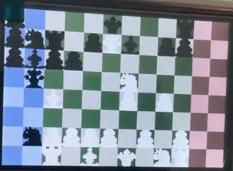
\includegraphics[width=0.45\textwidth]{images_zensiert/chessboard_display.png}}
    \caption{ChessBoard mode on the display}
    \label{fig:chessboard}
\end{figure}

\subsubsection*{InfoBoard}
The \emph{InfoBoard} is shown for 3 seconds after an input on the key matrix. It displays
the current input together with the result of the last rule check, respectively the
checkmate output.

\begin{figure}[H]
    \centering
    \fboxrule=1.2pt
    \fcolorbox{black}{white}{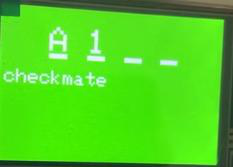
\includegraphics[width=0.45\textwidth]{images_zensiert/infoboard_display.png}}
    \caption{InfoBoard mode showing the input and a checkmate message}
    \label{fig:infoboard}
\end{figure}

\newpage

\subsection{Key Matrix Input Handling}

The class \texttt{Tastenmatrix} is a wrapper around the \texttt{Keyboard} class.

\subsubsection*{Evaluating the input}
The function \texttt{getKey()} reads the most recently pressed key. If it does not match
the required format, namely letter-number-letter-number, it is not used. The class
stores the four keys in an array which, once it is full, can be read out.

\subsubsection*{Getting the input}
With the functions \texttt{Koordinate getEingabe(uint8\_t key)} and
\texttt{Koordinate getEingabeChar(uint8\_t key)} a field can be requested from the key
array. Via the parameter \texttt{uint8\_t key} either the first or the second field can
be requested.

\begin{lstlisting}
function GET-KEY()
    k <- read last pressed key
    if k matches pattern Letter-Number-Letter-Number
        then store k in keyArray
    if keyArray is full              // 4 keys -> start field + target field
        then return keyArray
\end{lstlisting}

\subsection{Stockfish AI Implementation (Lichess)}

The move query is based on the open-source project Lichess, which makes its API freely
available to the public at \texttt{STOCKFISH\_API\_URL: https://stockfish.online/api/s/v2.php}.
With the function \texttt{getTurn()} the suggested move and the position evaluation can
be requested.

\subsection{WLAN Connection}

The WLAN connection is based on the \texttt{WifiManager} library. It provides a
ready-made website on which the WLAN password can be entered, so the Schachbot can
connect to the internet for the online AI mode without hard-coding any credentials.

\newpage

\subsection{Chess Rules Logic}

The chess-rules class is the core piece of our program. It not only calculates whether
a move is valid, it also provides information on \emph{why} a move is invalid, whether
the current position is checkmate or stalemate, and it calculates the moves when the
system is offline. Special rules such as \emph{en passant} and castling have been
implemented as well. This class was tested beforehand with a self-programmed Windows
application.

\begin{lstlisting}
function IS-VALID-MOVE(board, start, end)
    if no piece on start
        then return INVALID            // empty field
    if end not in LEGAL-MOVES(piece)
        then return INVALID            // illegal for piece
    if MOVING-INTO-CHECK(board, start, end)
        then return INVALID            // king in check
    return VALID

function GAME-STATE(board)
    if noLegalMoves and kingInCheck
        then return CHECKMATE
    if noLegalMoves and not kingInCheck
        then return STALEMATE
    return RUNNING
\end{lstlisting}

\begin{figure}[H]
    \centering
    \fboxrule=1.2pt
    \fcolorbox{black}{white}{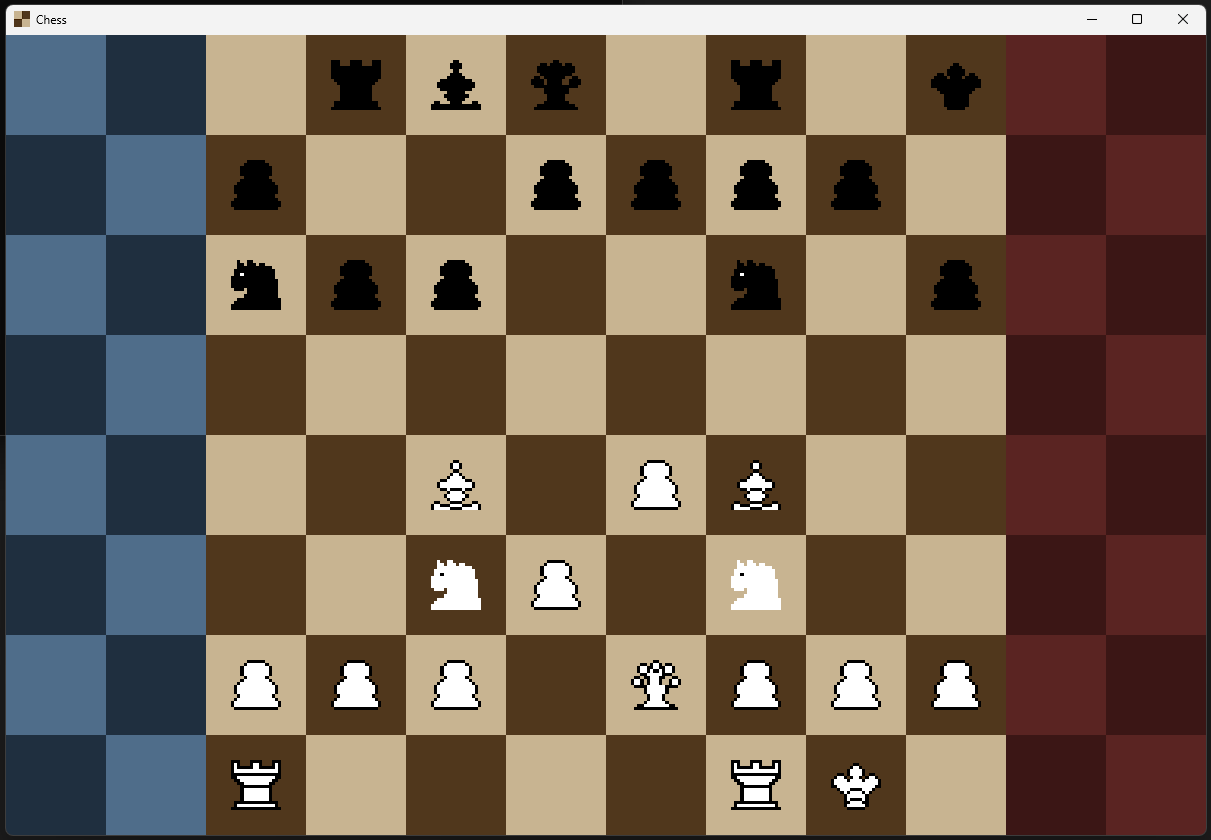
\includegraphics[width=0.8\textwidth]{images_zensiert/windows_application.png}}
    \caption{Self-programmed Windows application used to test the chess-rule logic}
    \label{fig:windows_app}
\end{figure}


\newpage

\section{Instruction manual}

\subsection{1. Materials Needed:}
\begin{itemize}
    \item The assembled Schachbot (gantry + board)
    \item A 230\,V wall socket
    \item Optionally a WLAN connection (for the Stockfish AI mode)
    \item Working eyes and a bit of chess knowledge
\end{itemize}

\subsection{2. Preparation Steps:}
\begin{enumerate}
    \item Place all chess pieces on their starting squares (as shown on the display).
    \item Plug the 24\,V power supply into the wall socket,the system powers up and homes the gantry.
    \item Wait until the display shows the starting position and ``Start Programm''.
    \item Choose your mode: play against a second player (1 vs.\ 1) or against the AI.
\end{enumerate}

\subsection{3. Playing a Move:}
\begin{itemize}
    \item Press the \textbf{start field} of the piece you want to move on your key matrix (e.g.\ \texttt{E2}).
    \item Press the \textbf{target field} (e.g.\ \texttt{E4}).
    \item If the move is legal, the gantry moves the piece automatically; if not, the display shows an error and nothing moves.
    \item In AI mode the gantry then plays the computer's answer by itself.
\end{itemize}

\subsection{4. Extra Commands / Inputs:}
Besides normal moves, the key matrix also accepts a few special commands. They are
entered just like a move (two ``fields''), but instead of a chess square you press a
fixed combination. The game mode is selected at the start of a game, while the
calibration command can be used at any time.

\textbf{Game mode selection:}
\begin{itemize}
    \item \texttt{G1 G1} --- \textbf{Game mode 1:} human vs.\ human (both players use their own key matrix).
    \item \texttt{G2 G2} --- \textbf{Game mode 2:} human vs.\ Stockfish (online AI, plays the best move).
    \item \texttt{G3 G3} --- \textbf{Game mode 3:} human vs.\ random moves (offline bot answers with a random legal move).
\end{itemize}

\textbf{Calibration / reset:}
\begin{itemize}
    \item \texttt{A1 A1} --- calibrates (homes) the gantry back to the \texttt{0/0} position
          and performs a logic reset: the electromagnet (coil) is switched off and the
          player can enter their move again.
\end{itemize}


\newpage

\section{Cost report}


\renewcommand{\arraystretch}{1.25}
\setlength{\tabcolsep}{4pt}
\noindent
\footnotesize
\begin{tabularx}{\textwidth}{|L{2.0cm}|L{2.6cm}|c|c|c|X|L{1.7cm}|}
\hline
\multicolumn{1}{|c|}{\textbf{Category}} & \multicolumn{1}{|c|}{\textbf{Parts}} & \multicolumn{1}{|c|}{\textbf{N}} & \multicolumn{1}{|c|}{\textbf{Cost}} & \multicolumn{1}{|c|}{\textbf{Total}} & \multicolumn{1}{|c|}{\textbf{Use Case}} & \multicolumn{1}{|c|}{\textbf{Store}} \\ \hline
\multicolumn{1}{|c|}{\textbf{I/O}} & Stop Button & 10 & 0,59~\euro & 5,90~\euro & 0/0 homing of the gantry & Amazon \\ \hline
 & Key Matrix & 2 & 0,00~\euro & 0,00~\euro & Input: moving the pieces & Armin/WE \\ \hline
 & LCD Display & 3 & 17,14~\euro & 51,42~\euro & Chessboard output / input output & Amazon \\ \hline
\multicolumn{1}{|c|}{\textbf{uC}} & ESP32 & 1 & 6,80~\euro & 6,80~\euro & Program & Berrybase \\ \hline
 & GPIO Expander & 1 & 9,00~\euro & 9,00~\euro & More GPIO pins & Berrybase \\ \hline
\multicolumn{1}{|c|}{\textbf{Power\-supply}} & Power Supply & 1 & 18,14~\euro & 18,14~\euro & Supply voltage & Amazon \\ \hline
 & Step-Down & 3 & 2,68~\euro & 8,04~\euro & ESP supply & Amazon \\ \hline
\multicolumn{1}{|c|}{\textbf{Magne\-tism}} & Coil & 1 & 8,05~\euro & 8,05~\euro & Dragging the pieces & Amazon \\ \hline
 & Neodym small & 50 & 0,14~\euro & 7,00~\euro & Small pieces permanent magnetism & Amazon \\ \hline
 & Neodym big & 20 & 0,25~\euro & 5,00~\euro & Large pieces permanent magnetism & Amazon \\ \hline
 & N-Channel Mosfet & 1 & 1,00~\euro & 1,00~\euro & Coil control & WE/Neuhold \\ \hline
\multicolumn{1}{|c|}{\textbf{Motors}} & Stepper Motors & 3 & 11,90~\euro & 35,70~\euro & Moving the gantry X/Y-axis & Amazon \\ \hline
 & Motor Driver & 3 & 7,68~\euro & 23,04~\euro & Controlling the motors & Amazon \\ \hline
\multicolumn{1}{|c|}{\textbf{Extras}} & AWG 18 Wire & 6 & 3,02~\euro & 18,12~\euro & Wiring & Amazon/WE \\ \hline
 & Filament Black & 1 & 10,58~\euro & 10,58~\euro & Emergency roll & Amazon \\ \hline
 & Filament White & 1 & 11,39~\euro & 11,39~\euro & Remaining 3D-print & Amazon \\ \hline
 & Filament Support & 1 & 17,50~\euro & 17,50~\euro & Supports & Amazon \\ \hline
 & Felt & 1 & 5,50~\euro & 5,50~\euro & Strong magnets & Hardware store \\ \hline
\multicolumn{1}{|c|}{\textbf{Circuit}} & Pin Headers & 1 & 0,00~\euro & 0,00~\euro & Mounting the components & WE \\ \hline
\multicolumn{1}{|c|}{\textbf{Gantry}} & Alu Profile 500mm & 2 & 24,25~\euro & 48,50~\euro & Roller structure 1 & 3D Proto \\ \hline
 & Roller + Screws & 1 & 2,50~\euro & 2,50~\euro & Roller for motor & 3D Proto \\ \hline
 & Alu Profile 1000mm & 1 & 16,50~\euro & 16,50~\euro & Roller structure 2 & 3D Proto \\ \hline
 & Roller + Screws & 1 & 2,40~\euro & 2,40~\euro & Roller for motor & 3D Proto \\ \hline
 & Coil holder & 1 & 4,00~\euro & 4,00~\euro & Holds coil & 3D Proto \\ \hline
\multicolumn{1}{|c|}{\textbf{Gantry (Extras)}} & Roller + Screws & 2 & 4,25~\euro & 8,50~\euro & Spare (can break) & 3D Proto \\ \hline
 & T-Slot Nuts & 1 & 3,50~\euro & 3,50~\euro & For the profile & 3D Proto \\ \hline
 & M4/M3 Screws & 5 & 1,36~\euro & 6,80~\euro & Extra screws for gantry parts & WE \\ \hline
 & Nuts & 7 & 1,71~\euro & 11,97~\euro & For fastening the screws & Link \\ \hline
 & Idler Pulley & 4 & 2,50~\euro & 10,00~\euro & Curve for belt & Link \\ \hline
 & Toothed Pulley & 2 & 3,00~\euro & 6,00~\euro & Converts motor rotation & Link \\ \hline
 & Belts & 2 & 2,00~\euro & 4,00~\euro & Drives XY-axis & Link \\ \hline
 & Cable Ties & 5 & 0,00~\euro & 0,00~\euro & For fastening the belt & WE \\ \hline
\multicolumn{1}{|c|}{\textbf{Case}} & M5 Screws & 100 & 0,20~\euro & 20,00~\euro & Mounting plate/plexiglass & OBI \\ \hline
 & M3,5 Screws & 100 & 0,00~\euro & 0,00~\euro & Mounting the wires & Kontakte \\ \hline
 & PlexiGlass & 1 & 0,00~\euro & 0,00~\euro & Roof/chessboard & Kontakte \\ \hline
 & Wooden Plate & 1 & 0,00~\euro & 0,00~\euro & Plate & Basement \\ \hline
\multicolumn{2}{|c|}{\textbf{Shipping cost:}} & \multicolumn{5}{c|}{\textbf{12,85~\euro}} \\ \hline
\multicolumn{2}{|c|}{\textbf{Total cost:}} & \multicolumn{5}{c|}{\textbf{413,70~\euro}} \\ \hline
\multicolumn{2}{|c|}{\textbf{Estimated cost:}} & \multicolumn{5}{c|}{\textbf{300,00~\euro}} \\ \hline
\end{tabularx}
\captionof{table}{Schachbot : Cost Report}
\label{tab:kosten}

\newpage

\section{Feedback}

\subsection{Learning Effects}

\subsubsection*{Time Management}
We learned that testing and debugging took significantly more time than expected. Our time management, especially towards the end of the project, could have been much better. We had to work many extra hours to complete everything. Additionally, we realized that ordering components earlier would have allowed us to make better use of our initial sessions.

\subsubsection*{Mechanics and the Gantry}
Building a precise 2D gantry from aluminium profiles, belts and 3D-printed parts taught us a lot about mechanical tolerances. Getting the steps-per-field (\texttt{FIELD\_STEPS}) exactly right and keeping the belts under proper tension was crucial for reliably hitting every square.

\subsubsection*{Magnetism}
Choosing the right combination of electromagnet and permanent magnets was harder than expected. The coupling had to be strong enough to drag a piece, but not so strong that neighbouring pieces were pulled along. The 5\,cm × 5\,cm field size and a small, precisely sized coil solved this.

\subsubsection*{Cost}
Choosing the right components before purchasing them is extremely important. We learned this the hard way, everything we bought incorrectly either resulted in additional costs or had to be resold. We also realized that a more expensive part is not necessarily better or suitable for our specific project needs.

\subsubsection*{Team Communication}
It is crucial to clearly define roles and responsibilities at the beginning of a project. Miscommunication and unclear task assignments led to avoidable conflicts and wasted valuable time.

\newpage

\subsection{What Went Badly}

\subsubsection*{Materials & Technology}
We didn't decide on the materials and technology early enough. Switching components and tools partway through the project cost us a lot of time and forced us to redo work we had already completed. Settling on these decisions at the start would have saved us significant effort.

\subsubsection*{Circuits}
We had to redesign the circuit because we forgot certain components. In some cases, we had to make spontaneous changes because we ran out of time to mill a new version.

\subsubsection*{Gantry Precision}
Getting the gantry to consistently land in the centre of every square took a lot of calibration. Small mechanical inaccuracies added up over the length of the rails and had to be compensated in software.

\subsubsection*{Team Structure}
There were moments of dissatisfaction with how team members handled their tasks. A clearer structure and better coordination would have helped avoid this.

\subsection{What Went Well}

\subsubsection*{Building the Casing}
The casing and the plexiglass playing field worked well and looked clean once assembled.

\subsubsection*{Building the 2D-Gantry}
The initial 2D-gantry worked in under 5 weeks, we were really fast on the mechanical side of things.

\subsubsection*{Constructing the Circuit}
One of our professors complimented the single-sided milled circuit layout, calling it beautiful. It was well-executed and organized.

\subsubsection*{Software Architecture}
Splitting the firmware into clearly separated classes (Gantry, Display, Tastenmatrix,
chess rules, API) paid off: every part could be tested on its own and then plugged into
the Main File without breaking the rest. The idea of letting the gantry compare an
``actual'' board against a ``target'' board kept the movement logic completely
independent from the chess logic, which made the whole system much easier to extend and
debug.

\newpage

\section{Sources and Programmes Used}

The following tools and programmes were used throughout the project:

\begin{itemize}
    \item \textbf{Onshape \& Fusion 360} --- for the complete 3D design of the gantry,
          mounts and casing parts.
    \item \textbf{Bambu Studio \& Bambu Lab A1} --- the 3D models were sliced in Bambu Studio
      and printed in-house on a Bambu Lab A1 printer to produce all custom parts.
    \item \textbf{EasyEDA} --- for designing the schematic and the single-sided PCB layout.
    \item \textbf{Microsoft Teams} --- for project planning, file sharing and team
          communication.
    \item \textbf{Google Datasheet} --- for tracking the budget.
    \item \textbf{\LaTeX{} (via Overleaf)} --- for writing and compiling this documentation.
    \item \textbf{GitHub} --- the complete source code is available at the link below.
    \item \textbf{Git} --- used for version control of the firmware, so changes could be
          tracked and the whole code base stayed in one central place.
    \item \textbf{Claude \& ChatGPT} --- used as a help for technical questions and translation.
    \item \textbf{Visual Studio Code} --- used to write and edit the C++ firmware for the ESP32 and used to write and edit the project presentation (reveal.js / HTML).
          HTML-based slide show.
     \item \textbf{Visual Studio} ---  for coding the Windows application
\end{itemize}

\subsection*{Source Code}

\begin{center}
The full firmware and project code is open source and can be found on GitHub, together
with this documentation and the project presentation. Feel free to use it. Scan the QR code or follow the link:
\end{center}

\begin{figure}[H]
    \centering
    \fboxrule=1.2pt
    \fcolorbox{black}{white}{
\includegraphics[width=0.40\textwidth]{images_zensiert/github_qr.jpeg}}
    \caption{QR code to the GitHub repository}
    \label{fig:github_qr}
\end{figure}

\begin{center}
    \url{https://github.com/ArminZechner/Schachbot}
\end{center}


\end{document}